\documentclass[letterpaper]{article} % DO NOT CHANGE THIS
% NeusymBridge uses double-blind review: keep the [submission] option (AAAI-27 Author Kit).
\usepackage[submission]{aaai2027}  % DO NOT CHANGE THIS
\usepackage{newtxmath}
\usepackage[hyphens]{url}  % DO NOT CHANGE THIS
\usepackage{graphicx} % DO NOT CHANGE THIS
\urlstyle{rm} % DO NOT CHANGE THIS
\def\UrlFont{\rm}  % DO NOT CHANGE THIS
\usepackage{natbib}  % DO NOT CHANGE THIS AND DO NOT ADD ANY OPTIONS TO IT
\usepackage{caption} % DO NOT CHANGE THIS AND DO NOT ADD ANY OPTIONS TO IT
\frenchspacing  % DO NOT CHANGE THIS
\usepackage{booktabs}
\usepackage{amsmath}
\usepackage{multirow}
\usepackage{array}
\usepackage{siunitx}
\usepackage[capitalize,noabbrev]{cleveref}
\newcommand{\clade}{\textsc{Clade}}
\pdfinfo{
/TemplateVersion (2027.1)
}
\setcounter{secnumdepth}{2}

\title{\clade{}: Category-Level Answering from Deficient Evidence\\in Retrieval-Augmented Language Models}
\author{Anonymous Submission}
\affiliations{}

\begin{document}

\maketitle

% \begin{abstract}
% Retrieval-augmented systems often provides a page that is true and relevant but contains only part of the answer, e.g. the question asks which disease a drug treats, and the page says \emph{hyperlipidemia}, where the answer is \emph{\textbf{familial} hyperlipidemia}. Work on sufficient context treats such pages as insufficient. We argue they form a distinct case, \emph{resolvable insufficiency}: the text cannot settle the answer, but its family name indexes a short candidate list in an ontology. Language models meet this phenomenon with \clade{} (category-level answering from deficient evidence): they answer instead of declining or looking further.  On 856 PrimeKG questions, a family-only page weakens the push toward ``not enough information'' by 13.8 points relative to a silent page (pooled over three 7--8B models, $p = 4\times10^{-5}$; significant for two of the three individually), and the freed answers are about as often wrong as right. A counterfactual edit isolates the cause: replacing the disease name with its family name lowers declines by 17.4 points relative to deleting the sentence. Confidence (AUROC 0.59--0.72 on family-only pages, against 0.73--0.87 on named pages), a 14B model (58\% precision, against 96\%) and an instruction to decline (more declines on every kind of page) all leave \clade{} in place. It replicates on species interactions from GloBI, with a taxonomy as the symbolic structure (900 questions; decline effect $-14.3$ points, $p = 10^{-9}$), where the freed answers are mostly wrong. Resolving the insufficiency is only partly solved: the ontology list holds the answer 98.5\% of the time once the family is known, but the family is found from the page only 19.8\% of the time, and a popularity prior beats both the model and literature evidence at choosing within it. The results locate where a neural reader should hand over to symbolic knowledge, and which steps of that handover remain open.
% \end{abstract}

% \begin{abstract}
% Retrieval-augmented systems often retrieve passages that are accurate and relevant, but state the answer at a coarser level of granularity than the question requires. For example, a question may ask which specific disease a drug treats (\emph{familial hyperlipidemia}), while the retrieved passage mentions the broader disease family (\emph{hyperlipidemia}). Prior work on context sufficiency treats such coarse passages simply as insufficient. We argue that they form a distinct case, which we call \emph{resolvable insufficiency}: text alone cannot settle the fine-grained answer, but the broader category it mentions maps to a short list of candidate answers in a domain ontology. When language models read these coarse, \emph{family-only} passages, they exhibit a phenomenon we call \clade{} (Category-Level Answering from Deficient Evidence): they answer instead of abstaining or searching further. Across 856 biomedical questions from PrimeKG, providing a family-only passage reduces abstention by 13.8 points compared to providing an uninformative passage. Moreover, the additional answers triggered by these coarse passages are wrong about half the time. A counterfactual experiment confirms the cause: replacing an exact disease name in a passage with its broader family name reduces abstention by 17.4 points compared to deleting the sentence. Simple fixes do not stop \clade{}. Filtering by model confidence (AUROC 0.59--0.72 on family-only passages versus 0.73--0.87 on exact-match passages), scaling to a bigger model (58\% precision versus 96\%), and explicitly instructing the model to abstain all fail to eliminate the problem. The same behavior appears in an ecological domain using species interactions from GloBI and a biological taxonomy (900 questions; abstention drop of $14.3$ points), where the extra guesses are mostly wrong. Finally, we test whether an ontology can resolve these coarse passages into exact answers. Once the correct family is known, the ontology's candidate list contains the true answer 98.5\% of the time. However, identifying the right family from the passage succeeds only 19.8\% of the time, and a simple popularity prior outperforms both the language model and literature co-mention counts when selecting the final answer. Together, our findings pinpoint where a neural reader should hand off to symbolic knowledge and which steps of that handoff remain unsolved.
% \end{abstract}

\begin{abstract}
Retrieval-augmented systems often retrieve passages that are accurate and relevant but state the answer at a coarser level of granularity than the question requires. For example, a question may ask which specific disease a drug treats (\emph{familial hyperlipidemia}), while the retrieved passage mentions the broader disease family (\emph{hyperlipidemia}). Prior work on context sufficiency treats such coarse passages simply as insufficient. We argue that they form a distinct case, which we call \emph{resolvable insufficiency}: text alone cannot settle the fine-grained answer, but the broader category it mentions maps to a short list of candidate answers in a domain ontology. When language models read these coarse, \emph{family-only} passages, they exhibit a phenomenon we call \clade{} (Category-Level Answering from Deficient Evidence): they answer instead of abstaining or searching further. On biomedical questions from PrimeKG, family-only passages reduce abstention by 13.8 points compared to uninformative passages, and the resulting guesses are wrong about half the time. A counterfactual test confirms the cause: replacing an exact disease name with its broader family name lowers abstention by 17.4 points compared to deleting the sentence. Simple fixes like confidence filtering, scaling to a larger model, and explicitly instructing the model to abstain cannot resolve \clade{}, and this replicates on ecological species interactions in GloBI. Finally, we test whether an ontology can turn coarse passages into exact answers. Given the correct family, an ontology list includes the true answer in 98.5\% of cases, but string matching finds that family on the page for only 19.8\%. Letting the model choose the family raises this to 30.0\% and end-to-end recovery from 10.0\% to 26.8\%. Overall, our results show when language models should stop guessing and consult an ontology, and highlight which steps of that process remain unsolved. Codes are available at: \url{https://anonymous.4open.science/r/CLADE}.
\end{abstract}

% \section{Introduction}

% \begin{figure*}[t]
% \centering
% 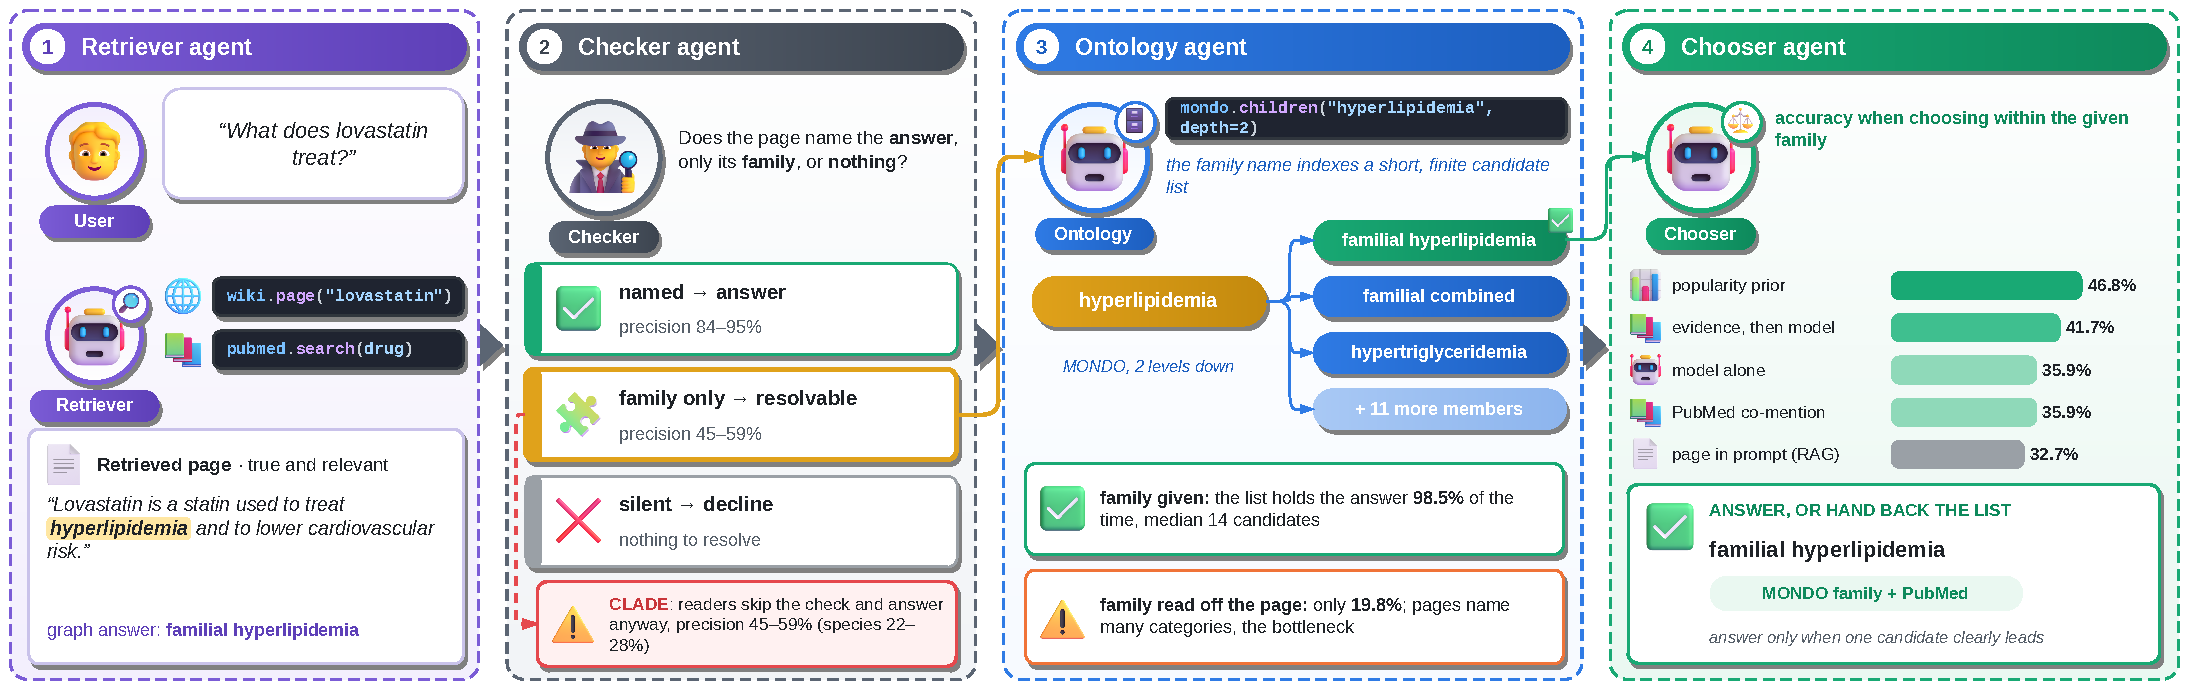
\includegraphics[width=\textwidth]{fig_concept.pdf}
% \caption{Resolvable insufficiency, drawn as a proposed agent workflow with the
% bottleneck we measure at each step. The dashed red path is \clade{}: the reader
% answers from the family-only page instead of handing it on. The retrieved page is true and relevant but
% names only the answer's family. A page-type check should route it away from
% answering; an ontology step turns the family name into a short candidate list;
% a chooser picks from it or hands the list back. Only the ontology step works
% reliably today.}
% \label{fig:concept}
% \end{figure*}

% A retrieval-augmented system answers a question by reading a page
% \citep{lewis2020rag}. Much recent work asks what the model should do when the
% page is not enough. The usual framing is binary: the context is sufficient or
% it is not \citep{joren2025sufficient}, and a well-behaved model answers in the
% first case and abstains in the second \citep{wen2025abstention}.

% Many pages fall between these cases in a structured way. Consider the question
% ``What does lovastatin treat?'' with the answer \emph{familial
% hyperlipidemia}, and a page that says ``lovastatin is used to treat
% hyperlipidemia'' (Figure~\ref{fig:concept}). The page is true and relevant. It
% rules out every disease that is not a hyperlipidemia. It does not say which
% one. A model can answer anyway, say ``not enough information,'' or look
% further. Looking further has a natural symbolic form: a disease ontology lists
% the members of the family, and each can be checked.

% We call this case \emph{resolvable insufficiency}. The page is insufficient,
% because it cannot settle the answer. It is resolvable in the sense of candidate-space reduction: the family name
% it does contain indexes a short, finite candidate set in a knowledge
% structure. Whether a system can then pick the right member is a separate
% question, which we also measure. When a model answers from such a page anyway,
% we call the behavior \clade{}: category-level answering from deficient
% evidence. This is the point where a neural reader and a symbolic resource
% have the most to offer each other, and it is common: in our data, text names
% the exact disease for only a minority of graph facts, and part of the rest is
% written at the family level.

% We ask three questions. How much of a biomedical knowledge graph does text
% name, and does a family name help a model at all? When a page names only the
% family, does a model stop declining, and are the answers it gives instead
% right? And can an ontology turn the family name back into the answer?

% Our contributions are:
% \begin{itemize}
% \item We define resolvable insufficiency and the failure it invites, \clade{},
% and measure it per fact, by
% classifying each page as naming the answer, naming only its family in the
% MONDO disease ontology, or naming nothing.
% \item We show that, pooled over three 7--8B models from different families, a
% family-only page weakens abstention relative to a silent page, using a design
% that compares each question with itself with and without the page, and that
% the answers it frees are about as often wrong as right, far less reliable than
% answers from a page that names the disease.
% \item We isolate the cause with a counterfactual edit of the same pages, show
% that confidence thresholds, a larger model and an instruction to decline do not
% remove the effect, and replicate it on species interactions with a taxonomy.
% \item We decompose ontology-based recovery into finding the family, listing
% its members, and choosing among them, and show that the first step is the
% bottleneck, while a popularity prior is a strong baseline for the last.
% \end{itemize}





\section{Introduction}

\begin{figure*}[t]
\centering
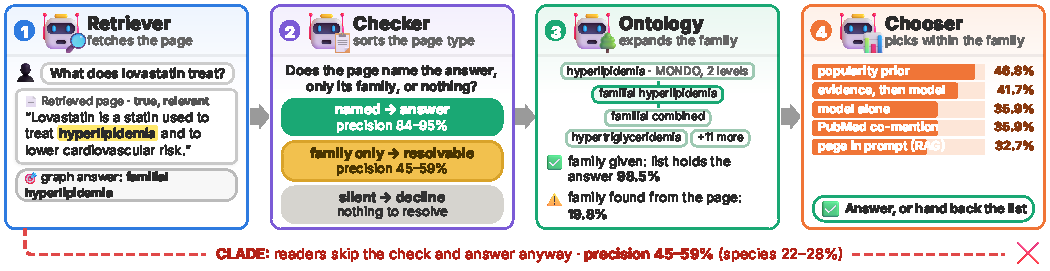
\includegraphics[width=\textwidth]{figures/fig_workflow.pdf}
\caption{\emph{Resolvable insufficiency} as an agent workflow, with the bottleneck we measure at each stage. The retrieved passage is accurate and relevant but names only the answer's family. A page-type check should send it to an ontology, which expands the family into a short candidate list for a chooser. The dashed red path is \clade{}: the model guesses from the family-only passage instead. Today only the ontology step works reliably.}
\label{fig:concept}
\end{figure*}

% Retrieval-augmented generation (RAG) systems answer questions by reading retrieved text \citep{lewis2020rag}. Recent works ask what a model should do when the retrieved text does not contain the complete answer. The usual framing is binary: the context is sufficient or it is not \citep{joren2025sufficient}, and a well-behaved model answers in the first case and abstains in the second \citep{wen2025abstention}. In practice, many retrieved passages fall between these two extremes. Consider the question, \emph{What disease does lovastatin treat?}, where the ground-truth answer is the specific condition \emph{familial hyperlipidemia}. Suppose the retriever returns a passage stating that \emph{lovastatin is used to treat hyperlipidemia} (~\ref{fig:concept}). This passage is both accurate and relevant. It rules out every disease outside the hyperlipidemia family, but it is too coarse to specify which exact subtype is meant. Faced with this passage, a system can guess a specific disease, abstain by saying there is not enough information, or look further. Looking further has a natural symbolic solution: a medical ontology lists the specific diseases within the hyperlipidemia family, and each candidate can then be checked.

% We call this phenomenon \emph{resolvable insufficiency}. The passage is insufficient on its own because it states the answer at a coarse category level rather than the fine-grained entity level required. However, it is resolvable because the coarse name maps directly to a small, finite set of candidate answers in a structured ontology. When a language model instead guesses a fine-grained answer directly from such coarse text, we call the behavior \clade{} (Category-Level Answering from Deficient Evidence). This setting represents a natural handoff point between neural readers and symbolic knowledge bases, and it occurs frequently in real text. In biomedical datasets, retrieved documents state the exact disease name for only a small fraction of knowledge-graph facts, while many of the remaining facts are described only at a broader family level. To facilitate our analysis, we group retrieved passages into three categories based on how specifically they describe the target answer:
% \begin{itemize}
% \item \emph{Named (exact-match) passages}, which explicitly mention the fine-grained target entity or an exact synonym.
% \item \emph{Family-only (coarse) passages}, which do not mention the specific answer, but mention a broader parent category (such as a disease family or biological genus) within two levels above the answer in an ontology.
% \item \emph{Silent (unmentioned) passages}, which talk about the query subject (e.g., the drug) but mention neither the specific answer nor its broader family.
% \end{itemize}

% \noindent Using the framework, we investigate three research questions:
% \begin{enumerate}
% \item How often do reference texts state fine-grained biomedical facts versus only coarse categories, and does a coarse category name help a language model answer on its own?
% \item When a retrieved passage provides only a coarse family name, does the model stop abstaining, and are the resulting answers accurate?
% \item Can a domain ontology bridge the gap by turning a coarse family mention into the exact fine-grained answer?
% \end{enumerate}

% Our main contributions are as follows:
% \begin{itemize}
% \item We define \emph{resolvable insufficiency} and the failure mode it triggers (\clade{}), and we measure how often reference texts describe knowledge-graph facts at an exact, coarse (\emph{family-only}), or unmentioned (\emph{silent}) level.
% \item Across three 7--8B language models from different model families, we show that coarse, family-only passages significantly reduce abstention compared to silent passages. By comparing each question against itself with and without the passage, we show that the extra answers triggered by family-only passages are wrong about half the time—far less reliable than answers based on named passages.
% \item We prove causality through counterfactual page edits, show that confidence filtering, larger model scale (14B), and explicit abstention prompts fail to prevent \clade{}, and replicate our findings in ecology using species interactions and a biological taxonomy.
% \item We break ontology-guided recovery into three steps—identifying the family on the page, listing its members, and selecting the final candidate—and show that identifying the right family on the page is the main bottleneck, while a simple popularity prior outperforms both the language model and literature co-mention counts at the final selection step.
% \end{itemize}


Retrieval-augmented generation (RAG) systems answer questions by reading retrieved text \citep{lewis2020rag}. Recent work asks what a model should do when that text does not contain the complete answer. The usual framing is binary: a passage is either sufficient or insufficient \citep{joren2025sufficient}, and a reliable model answers in the first case and abstains in the second \citep{wen2025abstention}. In practice, many retrieved passages fall between these two extremes. Consider the question \emph{What disease does lovastatin treat?}, where the true answer is the specific condition \emph{familial hyperlipidemia}. Suppose the retriever returns a passage stating that \emph{lovastatin is used to treat hyperlipidemia} (~\cref{fig:concept}). This passage is accurate and relevant. It rules out every disease outside the hyperlipidemia family, but it is too coarse to specify which exact subtype is meant. In this case, a system can guess a specific disease, abstain, or look further using a medical ontology that lists specific members of the hyperlipidemia family.

We call this phenomenon \emph{resolvable insufficiency}. The passage is insufficient on its own because it states the answer at a coarse category level rather than the required fine-grained entity level. Yet it is resolvable because the coarse name maps directly to a short, finite set of candidate answers in a structured ontology. When a model instead guesses a fine-grained answer directly from such coarse text, we name the behavior \clade{} (Category-Level Answering from Deficient Evidence). Although this setting occurs frequently in real text---biomedical documents state the exact disease name for only a small fraction of knowledge-graph facts while describing many others at the family level—prior work overlooks how coarse evidence affects model abstention. Rather than proposing a surface-level patch, this paper digs into the mechanics of this phenomenon to understand how coarse evidence misleads large language models (LLMs) and where a neural reader should hand off to symbolic knowledge.

To study this systematically, we group retrieved passages into three categories based on how specifically they describe the target answer: \emph{named} (exact-match) passages, which explicitly mention the fine-grained target entity or an exact synonym; \emph{family-only} (coarse) passages, which omit the specific answer but mention a broader parent category (such as a disease family or biological genus) within two levels above the answer in an ontology; and \emph{silent} (unmentioned) passages, which discuss the query subject (e.g., the drug) but mention neither the specific answer nor its broader family. Using this framework, we investigate three research questions: (1) how often reference texts state fine-grained biomedical facts versus coarse categories (and whether a coarse name helps a model on its own), (2) whether family-only passages cause models to stop abstaining and guess inaccurately, and (3) whether a domain ontology can turn a coarse family mention into the exact fine-grained answer. Our main contributions are as follows:
\begin{itemize}
\item We define \emph{resolvable insufficiency} and \clade{}, and measure how text states 1,800 PrimeKG facts and 23,694 GloBI interactions. Text omits the exact disease for 77.5--84.9\% of PrimeKG facts, and a family name alone gives the model no closed-book advantage.
\item On 856 PrimeKG questions and three 7--8B models, family-only passages cut abstention by 13.8 points relative to silent passages. About half of the extra answers are wrong, and precision falls from 84--95\% to 45--59\%.
\item Counterfactual edits show that the family name causes this drop ($-17.4$ points against deleting the sentence). Confidence filtering, a 14B model and an instruction to abstain do not stop \clade{}, and the effect replicates on 900 GloBI questions. In free text, no model gives the exact answer from a family-only passage.
\item On 410 family-only facts, an ontology list holds the answer 98.5\% of the time once the family is known, but string matching finds the family from the passage only 19.8\% of the time. A model that chooses the family raises this to 30.0\% and end-to-end recovery from 10.0\% to 26.8\%, and a popularity prior beats the model at choosing within the list.
\end{itemize}

% \section{Related Work}

% \paragraph{Insufficient context in RAG.}
% Retrieval failures are a recognized failure point of RAG systems
% \citep{barnett2024seven}. \citet{joren2025sufficient} introduce sufficient
% context as a lens on RAG errors, label contexts as sufficient or insufficient,
% and show that models often answer correctly even from insufficient context and
% hallucinate rather than abstain. They note that a context can narrow the answer
% without settling it, but treat it as insufficient. Models are also known to be
% distracted by irrelevant context \citep{shi2023distracted,yoran2024robust}, and
% \citet{setiawan2026misleading} show that misleading passages collapse
% prompt-based abstention while missing passages do not. Our case differs from
% both: the page is neither irrelevant nor misleading. It is correct and points
% in the right direction, and we show that this alone is enough to weaken
% abstention.

% \paragraph{Partial support and selective answering.}
% Self-RAG \citep{asai2024selfrag} trains a model to judge whether a passage
% fully or partially supports its output, and ALCE \citep{gao2023alce} grades
% citations by whether they support a claim. CRAG \citep{yan2024crag} scores
% retrieved documents and searches again when they are weak, and SURE-RAG
% \citep{qiu2026sure} verifies whether evidence is sufficient before answering.
% These methods recognize partial support, but not what kind of information is
% missing. A family name is a specific, structured kind of partial evidence:
% it says exactly which step is missing and where to look for it.

% \paragraph{Abstention.}
% Surveys and benchmarks document that models often answer when they should
% not \citep{wen2025abstention,kirichenko2025abstentionbench}, including in
% medicine \citep{machcha2026abstain}, and propose methods to detect knowledge
% gaps \citep{feng2024abstain,kadavath2022know}. These works measure whether a
% model declines. We measure which kind of evidence makes it stop declining.

% \paragraph{Ontologies and taxonomies in retrieval.}
% OG-RAG \citep{sharma2024ograg} grounds retrieval in a domain ontology, and
% TaSR-RAG \citep{sun2026tasr} uses a taxonomy to structure multi-hop retrieval.
% The broader program of combining language models with knowledge graphs is
% surveyed by \citet{pan2024unifying}, and neuro-symbolic AI more generally by
% \citet{garcez2023third}. These methods use symbolic structure for every query.
% We study the specific condition under which the page itself signals that a
% symbolic step is needed, and measure how far that step gets.

% \paragraph{What text contains.}
% \citet{mallen2023trust} and \citet{kandpal2023longtail} relate model knowledge
% to entity popularity and to the number of relevant pretraining documents, and
% LMEnt \citep{gottesman2026lment} traces entity mentions through a pretraining
% corpus. These studies work at the level of entities. We measure, for each fact,
% at what level of specificity the text names it.


\section{Related Work}

% \paragraph{Insufficient context in RAG.}
% Retrieval failures are a well-known weakness of RAG pipelines \citep{barnett2024seven}. \citet{joren2025sufficient} examine RAG errors through the lens of context sufficiency, labeling passages as either sufficient or insufficient. They observe that LLMs often hallucinate instead of abstaining when given insufficient context. Although they note that a passage can narrow down the space of possible answers without fully settling the question, their framework treats all such passages simply as insufficient. Prior work also shows that models are easily distracted by irrelevant text \citep{shi2023distracted,yoran2024robust}, and \citet{setiawan2026misleading} find that misleading passages cause prompt-based abstention to fail, whereas completely missing passages do not. Our setting differs from both irrelevant and misleading context. A coarse, family-only passage is factually correct and points in the right direction, yet we show that this partial relevance alone is enough to break abstention.

% \paragraph{Partial support and selective answering.}
% Several methods train or prompt models to evaluate evidence quality. Self-RAG \citep{asai2024selfrag} trains models to judge whether a passage fully or partially supports a generated claim, while ALCE \citep{gao2023alce} evaluates whether citations support model statements. CRAG \citep{yan2024crag} scores retrieved documents and triggers fresh web searches when support is weak, and SURE-RAG \citep{qiu2026sure} verifies context sufficiency before generating an answer. While these systems recognize that support can be partial, they do not identify what specific piece of information is missing. A coarse category mention is a structured form of partial evidence: it indicates that entity-level specificity is missing and points to where the candidates live in an ontology.

% \paragraph{Abstention in language models.}
% Recent surveys and benchmarks show that language models frequently guess when they should abstain \citep{wen2025abstention,kirichenko2025abstentionbench}, including in high-stakes clinical settings \citep{machcha2026abstain}. Prior methods focus on detecting when a model lacks knowledge \citep{kadavath2022know,feng2024abstain}. While those studies measure whether a model abstains overall, we isolate what kind of retrieved evidence tricks a model into abandoning abstention.

% \paragraph{Ontologies and taxonomies in retrieval.}
% Several RAG architectures incorporate structured knowledge. OG-RAG \citep{sharma2024ograg} grounds retrieval in domain ontologies, and TaSR-RAG \citep{sun2026tasr} uses taxonomies to guide multi-hop retrieval. Broader efforts to combine language models with knowledge graphs and symbolic reasoning are surveyed by \citet{pan2024unifying} and \citet{garcez2023third}. Unlike pipelines that invoke symbolic structures on every query, we identify the exact condition where a retrieved text signals the need for an ontology lookup, and we measure where that symbolic handoff succeeds or fails.

% \paragraph{Fact coverage in text corpora.}
% Prior work links a language model's parametric knowledge to how often entities appear in pretraining corpora \citep{mallen2023trust,kandpal2023longtail,gottesman2026lment}. Whereas those studies count mentions of individual entities, we measure the level of granularity at which reference texts state relational facts.


\paragraph{Insufficient context.}
Retrieval failures are a common weakness in RAG systems \citep{barnett2024seven}. \citet{joren2025sufficient} study the errors through the lens of context sufficiency. They label retrieved passages as either sufficient or insufficient and find that LLMs often hallucinate instead of abstaining when context is insufficient. Although they note that a passage can narrow down the answer without fully settling it, they group all such cases under insufficient context. Prior work also shows that models are easily thrown off by irrelevant text \citep{shi2023distracted,yoran2024robust}, and \citet{setiawan2026misleading} show that misleading passages cause prompt-based abstention to fail, whereas missing passages do not. Our focus, \emph{resolvable insufficiency}, differs from both irrelevant and misleading context. A coarse passage is factually accurate and points in the right direction, yet this partial relevance is enough to trigger \clade{} and break abstention.

\paragraph{Partial evidence.}
To handle imperfect passages, several methods train or prompt models to grade evidence quality. Self-RAG \citep{asai2024selfrag} trains a model to judge whether a passage fully or partially supports a generated answer, and ALCE \citep{gao2023alce} checks whether citations back up model claims. Similarly, CRAG \citep{yan2024crag} scores retrieved documents to trigger new searches when support is weak, and SURE-RAG \citep{qiu2026sure} checks whether context is sufficient before answering. While these methods detect that support is partial, they do not identify what kind of information is missing. A coarse mention is a structured form of partial evidence: it shows that fine-grained entity detail is missing and indicates where to find the candidate answers in an ontology.

\paragraph{Abstention.}
When evidence falls short and cannot be resolved, a reliable model should abstain. Recent surveys and benchmarks show that models often guess when they should hold back \citep{wen2025abstention,kirichenko2025abstentionbench}, including in clinical settings \citep{machcha2026abstain}. Most existing methods focus on detecting when a model lacks knowledge so it can decline to answer \citep{kadavath2022know,feng2024abstain}. While those studies measure whether a model abstains overall, we test how the granularity of retrieved evidence (\emph{named}, \emph{family-only}, \emph{silent}) causes a model to stop abstaining and guess.

\paragraph{Ontologies in RAG.}
Rather than guessing or abstaining on a coarse passage, a system can consult a structured ontology. Recent RAG systems use symbolic structures to guide retrieval: OG-RAG \citep{sharma2024ograg} grounds retrieval in domain ontologies, and TaSR-RAG \citep{sun2026tasr} uses taxonomies for multi-hop retrieval. Broader work on combining LLMs with knowledge graphs and symbolic reasoning is surveyed by \citet{pan2024unifying} and \citet{garcez2023third}. Unlike pipelines that query an ontology on every question, we study the specific case where a coarse passage calls for an ontology lookup. We also measure each step of the pipeline: extracting the family, listing its members, and picking the final answer; then we check where the process breaks down.

\paragraph{Fact coverage in text.}
Our analysis also connects to work on what reference and pretraining texts actually state. \citet{mallen2023trust} and \citet{kandpal2023longtail} link a model's closed-book knowledge to entity popularity and document counts, while LMEnt \citep{gottesman2026lment} tracks entity mentions across pretraining data. Whereas those studies count mentions of individual entities, we measure how often reference texts state relational facts at an exact (\emph{named}) level versus a coarse (\emph{family-only}) level.

\paragraph{Fine-grained biology.}
Biology shows the same gap between coarse and fine answers. On Bio-VQA, taxonomic accuracy falls from 0.72 at phylum to 0.12 at species \citep{rayeed2027biovqa}. And models lose accuracy from genus to species \citep{rayeed2025beetleverse} even on curated specimen images with validated traits \citep{rayeed2026beetles}. Knowledge-based VQA benchmarks also contain answers that their corpus does not support \citep{ma2026pitfalls}. We investigate the text side of this gap: a page that names the genus or family but not the answer.


% \section{Setting and Data}

% \paragraph{Facts and ontology.}
% We use drug--disease edges from PrimeKG \citep{chandak2023primekg}, whose
% indication and contraindication relations come from DrugCentral. Diseases are
% identified by MONDO \citep{vasilevsky2022mondo}, which we rebuild as a directed
% child-to-parent table of 17,801 edges over 11,788 diseases; 3,182 parent terms
% have two or more children.

% \paragraph{Text.}
% For each drug we use its English Wikipedia article and a set of PubMed
% abstracts retrieved per drug with a separate query budget for each relation.
% Wikipedia markup is cleaned before use: templates, tables, reference tags and
% file links are removed, and links are reduced to their visible text.

% \paragraph{How a page names a fact.}
% For each edge we classify the drug's text into one of three groups.
% \emph{Named}: the text contains the disease's exact name or an alternative
% name taken from Wikipedia redirects to the disease's article, which include
% synonyms, lay terms and abbreviations. \emph{Family-only}: the text contains
% none of these but names one of the disease's MONDO ancestors within two
% levels. \emph{Silent}: the text names neither. To separate
% real mentions from coincidence, each edge is paired with three diseases the
% drug has no relation to, and the same matcher is run on them.

% \subsection{How Much Does Text Reach?}

% We first measure, on 1,800 PrimeKG edges (600 per relation for indication,
% contraindication and off-label use), how often the drug's Wikipedia article
% names the disease and how often a model knows the fact closed book. The model
% picks the true disease from five options by mean token log-probability.

% \begin{table}[t]
% \centering
% \small
% \begin{tabular}{lcc}
% \toprule
%  & Model knows it & Model does not \\
% \midrule
% Text names it & 5.2 & 6.2 \\
% Text does not & 22.2 & 66.4 \\
% \bottomrule
% \end{tabular}
% \caption{Share of 1,800 PrimeKG facts (\%) by whether Wikipedia names the
% disease and whether Qwen2.5 0.5B picks it from five options closed book.}
% \label{tab:boxes}
% \end{table}

% Table~\ref{tab:boxes} crosses the two; here ``names it'' means the exact or an
% alternative name, so facts named only by their family count as not named. For
% two thirds of the facts, the text does not name the disease and the model does
% not know the answer. The ``knows it anyway'' cell is mostly chance: accuracy on
% facts the text does not name is 25.1\% against a 20\% chance rate, about 6\%
% above chance after correction. A second corpus helps little: on a separate
% sample measured in both corpora, the share not named is 84.9\% in Wikipedia,
% 81.1\% in PubMed abstracts and 77.5\% in both.

% \paragraph{A family name alone does not help the model.}
% If a family name carried useful signal, facts whose text names only the family
% would be easier for the model than facts whose text is silent. Testing this
% inside each relation and pooling with relation as a stratum on Qwen2.5-7B,
% family-only facts differ sharply from named facts (Mantel--Haenszel odds ratio
% 0.27, 95\% CI 0.17--0.43, $p = 9\times10^{-9}$) and not measurably from
% silent facts (odds ratio 1.10, 95\% CI 0.80--1.53, $p = 0.61$). The cleanest
% case is indications at 7B: 44.68\% correct for family-only facts against
% 43.95\% for silent facts. For contraindications the figures are 18.75\% and
% 23.35\%. An exact name raises the odds that the model knows a fact about
% 3.7-fold; a family name gives no measurable help on its own.

% This motivates the rest of the paper. The family name is the most common form
% of partial evidence in this data, and the model cannot use it by itself. The
% question is what happens when such a page is placed in front of the model at
% answer time, and whether a symbolic step can make use of it.



% \section{Data and Problem Setup}

% \paragraph{Knowledge graphs and ontologies.}
% Our primary benchmark uses drug-disease relations from PrimeKG \citep{chandak2023primekg}, which draws clinical indication and contraindication facts from DrugCentral. Each disease is linked to the MONDO Disease Ontology \citep{vasilevsky2022mondo}. We reconstruct MONDO as a directed child-to-parent hierarchy, with \num{17801} edges across \num{11788} diseases, in which \num{3182} parent categories have two or more child diseases. We exclude parents with more than 400 descendants (e.g. \emph{disease} or \emph{disorder}), since naming them gives no usable hint. To test whether our findings generalize beyond medicine, we also evaluate species-interaction facts from Global Biotic Interactions (GloBI; \citealt{poelen2014globi}). In GloBI, we examine four ecological relations (\emph{eats}, \emph{preys on}, \emph{parasite of}, and \emph{pollinates}) and use the Tree-of-Life biological taxonomy (\emph{species}, \emph{genus}, \emph{family}) as the hierarchy. We keep only species-level names on both sides of an edge, which leaves \num{457386} species-to-species edges. Table~\ref{tab:data} summarizes both domains. The two hierarchies have the same shape: the median family has three members, so a family name narrows the answer to a short list but does not settle it.

% \begin{table}[t]
\centering
\small
\setlength{\tabcolsep}{3.5pt}
\begin{tabular}{@{}lrr@{}}
\toprule
 & PrimeKG & GloBI \\
\midrule
Source records & 8,100,498 & 7,822,670 \\
\midrule
\multirow{4}{*}{Edges} & indication 9,388 & eats 235,960 \\
 & contraind.\ 30,675 & preys on 87,678 \\
 & off-label 2,568 & parasite of 117,894 \\
 & & pollinates 15,854 \\
\midrule
Hierarchy & MONDO & GloBI taxonomy \\
\quad child--parent links & 17,801 & 77,852 \\
\quad families, $\ge$2 members & 3,182 & 8,370 \\
\quad median / max size & 3 / 150 & 3 / 315 \\
\midrule
Text & Wiki.\ + PubMed & Wikipedia \\
\quad sources with text & 574 drugs & 5,425 species \\
\quad facts measured & 3,444 & 23,694 \\
Questions & 856 & 900 \\
\bottomrule
\end{tabular}
\caption{Data for both domains. PrimeKG links drugs to diseases, and MONDO groups diseases into families. GloBI links species to species, and its taxonomy groups species into genera. A \emph{family} is a parent with two or more children. \emph{Facts measured} are edges we check for a mention of the answer.}
\label{tab:data}
\end{table}


% \paragraph{Reference text corpora.}
% For each drug in PrimeKG, we collect its English Wikipedia article and a set of PubMed abstracts retrieved using separate query budgets for indications and contraindications. For each organism in GloBI, we use the consumer species' English Wikipedia article, skipping stubs shorter than 3,000 characters. All Wikipedia articles are stripped of markup, templates, infoboxes, tables, reference tags, and file links, leaving only the plain article text.

% \paragraph{Evidence granularity.}
% For any given fact (e.g. a drug treating a specific disease), we classify the retrieved text into one of three granularity levels:
% \begin{itemize}
% \item \textbf{Named (exact-match):} The passage contains the exact name of the target disease (or target species), or a known synonym, or abbreviation from Wikipedia redirect titles.
% \item \textbf{Family-only (coarse):} The passage does not contain the exact answer or synonyms, but mentions a broader parent category within two levels of the answer in the hierarchy.
% \item \textbf{Silent (unmentioned):} The passage mentions neither the exact answer nor any parent category within two levels.
% \end{itemize}

% To verify that matches reflect genuine mentions rather than chance word overlap, we pair each fact with three unrelated diseases (or species) from the same relation and run the same text matcher as a baseline control. On a separate sample of 1,800 PrimeKG facts measured in Wikipedia, the unrelated diseases are named in 0.9-1.4\% of articles and named or matched by family in 1.8-3.3\%, against 6.7-19.3\% and 9.3-34.7\% for the true disease across the three relations. Matches therefore track the fact, not the size of the name set.

% \paragraph{How often does text have the exact answer?}

% \begin{table}[t]
\centering
\small
\setlength{\tabcolsep}{4pt}
\begin{tabular}{@{}lrrrrr@{}}
\toprule
 & & \multicolumn{2}{c}{Text names it} & \multicolumn{2}{c}{Text does not} \\
\cmidrule(lr){3-4}\cmidrule(l){5-6}
Relation & $n$ & knows & not & knows & not \\
\midrule
Indication & 600 & 9.7 & 7.2 & 21.8 & 61.3 \\
Contraind. & 600 & 1.5 & 5.2 & 20.7 & 72.7 \\
Off-label & 600 & 4.3 & 6.2 & 24.2 & 65.3 \\
\midrule
All & 1,800 & 5.2 & 6.2 & 22.2 & \textbf{66.4} \\
\bottomrule
\end{tabular}
\caption{Share of PrimeKG facts (\%) by whether the drug's Wikipedia article
names the disease and whether Qwen2.5 0.5B picks it from five options closed
book (``knows'').}
\label{tab:boxes}
\end{table}


% Before testing RAG, we test how often reference texts contain the fine-grained answer and how often an LLM knows the fact without any retrieval (closed book). We sample 1,800 PrimeKG facts (600 each for indication, contraindication, and off-label use) and test whether Qwen2.5 0.5B can pick the true disease from five options based on mean token log-probability. ~\cref{tab:boxes} cross-tabulates closed-book model accuracy against whether the drug's Wikipedia page names the exact disease. Here, coarse (\emph{family-only}) mentions are grouped under \emph{Text does not name it}. For two-thirds of the facts (66.4\%), Wikipedia does not state the exact disease and the model does not know the answer. The share is highest for contraindications (72.7\%), where Wikipedia names the disease for only 6.7\% of facts. Even when the model selects the right option without text (22.2\%), much of that success is random guessing: closed-book accuracy on unnamed facts is 25.1\% compared to a 20.0\% five-choice guessing rate, which corresponds to only about 5\% above-chance knowledge.

% \begin{table}[t]
\centering
\small
\setlength{\tabcolsep}{4pt}
\begin{tabular}{@{}llrrrr@{}}
\toprule
Relation & Text & $n$ & Named & Family & Silent \\
\midrule
\multirow{3}{*}{Indication} & Wikipedia & 1,722 & 20.3 & 15.5 & 64.2 \\
 & PubMed & 1,722 & 26.3 & 18.6 & 55.1 \\
 & both & 1,722 & 29.0 & 19.7 & 51.3 \\
\midrule
\multirow{3}{*}{Contraind.} & Wikipedia & 1,722 & 9.8 & 4.1 & 86.1 \\
 & PubMed & 1,722 & 11.4 & 5.4 & 83.2 \\
 & both & 1,722 & 15.9 & 6.9 & 77.2 \\
\midrule
PrimeKG & both & 3,444 & 22.5 & 13.3 & 64.2 \\
\midrule
Eats & Wikipedia & 8,000 & 4.0 & 6.6 & 89.3 \\
Preys on & Wikipedia & 8,000 & 2.2 & 4.4 & 93.4 \\
Parasite of & Wikipedia & 2,389 & 12.5 & 15.5 & 72.0 \\
Pollinates & Wikipedia & 5,305 & 2.2 & 8.0 & 89.7 \\
\midrule
GloBI & Wikipedia & 23,694 & 3.9 & 7.1 & 89.1 \\
\bottomrule
\end{tabular}
\caption{Share of knowledge-graph facts whose text names the answer, names only its family, or names neither. PrimeKG uses 574 drugs with three facts of each relation.}
\label{tab:coverage}
\end{table}


% Adding a second biomedical corpus (\emph{PubMed}) barely changes this. Table~\ref{tab:coverage} measures a drug-matched sample of 574 drugs, each with three indications and three contraindications. The exact disease is missing in 84.9\% of Wikipedia articles, 81.1\% of PubMed abstract sets, and 77.5\% of both corpora combined. Indications are named about twice as often as contraindications in every corpus (29.0\% vs.\ 15.9\% in both combined). Family-only text covers 13.3\% of PrimeKG facts, more than half as many as are named (22.5\%). In GloBI, exact species mentions are even rarer (3.9\%), while coarse genus or family mentions account for nearly twice as many facts (7.1\%). The pattern holds in every GloBI relation, and \emph{parasite of} has the most family-only text (15.5\%).

% \paragraph{Coarse mentions do not reflect stronger closed-book knowledge.}
% One might wonder whether facts described at the family level in text are simply easier facts that the model already knows. If a coarse mention reflected easier underlying facts, then models tested closed book should perform better on family-only facts than on silent facts. We test this on Qwen2.5-7B across all relations using Mantel--Haenszel stratified odds ratios (Table~\ref{tab:closedbook}). Closed-book accuracy on family-only facts is much lower than on named facts (odds ratio $0.27$, 95\% CI $0.17$--$0.43$, $p = 9\times10^{-9}$) and is statistically indistinguishable from silent facts (odds ratio $1.10$, 95\% CI $0.80$--$1.53$, $p = 0.61$). For drug indications, Qwen2.5-7B answers 44.7\% of family-only facts correctly closed book versus 44.0\% of silent facts; for contraindications, the rates are 18.8\% versus 23.4\%. While an exact mention in Wikipedia corresponds to a 3.7-fold increase in the odds that the model knows the fact closed book, a coarse family mention provides no measurable advantage on its own.

% \begin{table}[t]
\centering
\small
\setlength{\tabcolsep}{4pt}
\begin{tabular}{@{}lrrr@{}}
\toprule
Relation & Named & Family only & Silent \\
\midrule
Indication & 84.2 {\scriptsize(101)} & 44.7 {\scriptsize(94)} & 44.0 {\scriptsize(405)} \\
Contraind. & 32.5 {\scriptsize(40)} & 18.8 {\scriptsize(16)} & 23.4 {\scriptsize(544)} \\
Off-label & 57.1 {\scriptsize(63)} & 37.5 {\scriptsize(72)} & 31.6 {\scriptsize(465)} \\
\midrule
All & 65.7 {\scriptsize(204)} & 39.6 {\scriptsize(182)} & 32.0 {\scriptsize(1,414)} \\
\bottomrule
\end{tabular}
\caption{Closed-book accuracy of Qwen2.5-7B by what the drug's Wikipedia page says about the answer. Chance is 20\%.}
\label{tab:closedbook}
\end{table}


% This observation motivates the rest of our study. Coarse category mentions are the most common form of partial evidence in reference text, yet they do not correspond to facts the model already knows. We therefore ask what happens when a coarse, family-only passage is shown to the model at inference time, and whether a symbolic ontology can help recover the exact answer.



% \section{Data and Problem Setup}

% We use drug-disease facts from PrimeKG, linking each disease to the MONDO ontology. We rebuild MONDO as a hierarchy of 17,801 edges across 11,788 diseases, excluding parents with over 400 descendants. To test generalizability, we also evaluate species interactions from GloBI, keeping 457,386 species-to-species edges across four ecological relations. For each entity, we collect its English Wikipedia article (and PubMed abstracts for drugs) and strip all markup.

% \begin{table}[t]
\centering
\small
\setlength{\tabcolsep}{3.5pt}
\begin{tabular}{@{}lrr@{}}
\toprule
 & PrimeKG & GloBI \\
\midrule
Source records & 8,100,498 & 7,822,670 \\
\midrule
\multirow{4}{*}{Edges} & indication 9,388 & eats 235,960 \\
 & contraind.\ 30,675 & preys on 87,678 \\
 & off-label 2,568 & parasite of 117,894 \\
 & & pollinates 15,854 \\
\midrule
Hierarchy & MONDO & GloBI taxonomy \\
\quad child--parent links & 17,801 & 77,852 \\
\quad families, $\ge$2 members & 3,182 & 8,370 \\
\quad median / max size & 3 / 150 & 3 / 315 \\
\midrule
Text & Wiki.\ + PubMed & Wikipedia \\
\quad sources with text & 574 drugs & 5,425 species \\
\quad facts measured & 3,444 & 23,694 \\
Questions & 856 & 900 \\
\bottomrule
\end{tabular}
\caption{Data for both domains. PrimeKG links drugs to diseases, and MONDO groups diseases into families. GloBI links species to species, and its taxonomy groups species into genera. A \emph{family} is a parent with two or more children. \emph{Facts measured} are edges we check for a mention of the answer.}
\label{tab:data}
\end{table}


% We classify retrieved text into three granularity levels:
% \begin{itemize}
% \item \textbf{Named:} The passage contains the exact name or a known redirect synonym.
% \item \textbf{Family-only:} The passage lacks the exact name but mentions a parent category within two levels above in the hierarchy.
% \item \textbf{Silent:} The passage mentions neither.
% \end{itemize}

% Control tests with unrelated disease pairs confirm that text matches track the actual fact rather than name-set size (false matches occur in only 0.9--1.4\% of articles).

% We test how often text states the exact answer and how well Qwen2.5 0.5B knows facts closed book using 1,800 PrimeKG facts. As shown in Table~\ref{tab:boxes} and Table~\ref{tab:coverage}, Wikipedia completely misses the exact disease for 84.9\% of facts (77.5\% across both Wikipedia and PubMed). For two-thirds of facts (66.4\%), the text is missing and the model does not know the answer. 

% \begin{table}[t]
\centering
\small
\setlength{\tabcolsep}{4pt}
\begin{tabular}{@{}lrrrrr@{}}
\toprule
 & & \multicolumn{2}{c}{Text names it} & \multicolumn{2}{c}{Text does not} \\
\cmidrule(lr){3-4}\cmidrule(l){5-6}
Relation & $n$ & knows & not & knows & not \\
\midrule
Indication & 600 & 9.7 & 7.2 & 21.8 & 61.3 \\
Contraind. & 600 & 1.5 & 5.2 & 20.7 & 72.7 \\
Off-label & 600 & 4.3 & 6.2 & 24.2 & 65.3 \\
\midrule
All & 1,800 & 5.2 & 6.2 & 22.2 & \textbf{66.4} \\
\bottomrule
\end{tabular}
\caption{Share of PrimeKG facts (\%) by whether the drug's Wikipedia article
names the disease and whether Qwen2.5 0.5B picks it from five options closed
book (``knows'').}
\label{tab:boxes}
\end{table}

% \begin{table}[t]
\centering
\small
\setlength{\tabcolsep}{4pt}
\begin{tabular}{@{}llrrrr@{}}
\toprule
Relation & Text & $n$ & Named & Family & Silent \\
\midrule
\multirow{3}{*}{Indication} & Wikipedia & 1,722 & 20.3 & 15.5 & 64.2 \\
 & PubMed & 1,722 & 26.3 & 18.6 & 55.1 \\
 & both & 1,722 & 29.0 & 19.7 & 51.3 \\
\midrule
\multirow{3}{*}{Contraind.} & Wikipedia & 1,722 & 9.8 & 4.1 & 86.1 \\
 & PubMed & 1,722 & 11.4 & 5.4 & 83.2 \\
 & both & 1,722 & 15.9 & 6.9 & 77.2 \\
\midrule
PrimeKG & both & 3,444 & 22.5 & 13.3 & 64.2 \\
\midrule
Eats & Wikipedia & 8,000 & 4.0 & 6.6 & 89.3 \\
Preys on & Wikipedia & 8,000 & 2.2 & 4.4 & 93.4 \\
Parasite of & Wikipedia & 2,389 & 12.5 & 15.5 & 72.0 \\
Pollinates & Wikipedia & 5,305 & 2.2 & 8.0 & 89.7 \\
\midrule
GloBI & Wikipedia & 23,694 & 3.9 & 7.1 & 89.1 \\
\bottomrule
\end{tabular}
\caption{Share of knowledge-graph facts whose text names the answer, names only its family, or names neither. PrimeKG uses 574 drugs with three facts of each relation.}
\label{tab:coverage}
\end{table}


% Crucially, family-only mentions do not reflect stronger closed-book knowledge. Tested on Qwen2.5-7B, closed-book accuracy on family-only facts is much lower than on named facts (odds ratio $0.27$, $p = 9\times10^{-9}$) and indistinguishable from silent facts (odds ratio $1.10$, $p = 0.61$). While an exact name in Wikipedia increases the odds that a model knows a fact 3.7-fold, a family name provides no measurable advantage on its own. 

% \begin{table}[t]
\centering
\small
\setlength{\tabcolsep}{4pt}
\begin{tabular}{@{}lrrr@{}}
\toprule
Relation & Named & Family only & Silent \\
\midrule
Indication & 84.2 {\scriptsize(101)} & 44.7 {\scriptsize(94)} & 44.0 {\scriptsize(405)} \\
Contraind. & 32.5 {\scriptsize(40)} & 18.8 {\scriptsize(16)} & 23.4 {\scriptsize(544)} \\
Off-label & 57.1 {\scriptsize(63)} & 37.5 {\scriptsize(72)} & 31.6 {\scriptsize(465)} \\
\midrule
All & 65.7 {\scriptsize(204)} & 39.6 {\scriptsize(182)} & 32.0 {\scriptsize(1,414)} \\
\bottomrule
\end{tabular}
\caption{Closed-book accuracy of Qwen2.5-7B by what the drug's Wikipedia page says about the answer. Chance is 20\%.}
\label{tab:closedbook}
\end{table}


% Coarse mentions are common partial evidence, which prompts us to test how models handle them at inference time and whether a symbolic ontology can recover the exact answer.

\section{Data and Problem Setup}

\paragraph{Knowledge graphs and ontologies.}
We use drug-disease relations from PrimeKG, linked to the MONDO Disease Ontology. We reconstruct MONDO into 17,801 edges across 11,788 diseases (excluding parents with $>$\num{400} descendants). To test generalizability beyond medicine, we evaluate species interactions from GloBI, using 457,386 species-to-species edges across four relations (\emph{eats}, \emph{preys on}, \emph{parasite of}, \emph{pollinates}) with GloBI's taxonomy (species, genus, family) as the hierarchy.~\cref{tab:data} summarizes both domains.

\begin{table}[t]
\centering
\small
\setlength{\tabcolsep}{3.5pt}
\begin{tabular}{@{}lrr@{}}
\toprule
 & PrimeKG & GloBI \\
\midrule
Source records & 8,100,498 & 7,822,670 \\
\midrule
\multirow{4}{*}{Edges} & indication 9,388 & eats 235,960 \\
 & contraind.\ 30,675 & preys on 87,678 \\
 & off-label 2,568 & parasite of 117,894 \\
 & & pollinates 15,854 \\
\midrule
Hierarchy & MONDO & GloBI taxonomy \\
\quad child--parent links & 17,801 & 77,852 \\
\quad families, $\ge$2 members & 3,182 & 8,370 \\
\quad median / max size & 3 / 150 & 3 / 315 \\
\midrule
Text & Wiki.\ + PubMed & Wikipedia \\
\quad sources with text & 574 drugs & 5,425 species \\
\quad facts measured & 3,444 & 23,694 \\
Questions & 856 & 900 \\
\bottomrule
\end{tabular}
\caption{Data for both domains. PrimeKG links drugs to diseases, and MONDO groups diseases into families. GloBI links species to species, and its taxonomy groups species into genera. A \emph{family} is a parent with two or more children. \emph{Facts measured} are edges we check for a mention of the answer.}
\label{tab:data}
\end{table}


\paragraph{Reference text corpora.}
For PrimeKG drugs, we use English Wikipedia articles and PubMed abstracts. For GloBI organisms, we use species' Wikipedia articles (dropping stubs $<$\num{3000} characters). All articles are stripped of markup, templates, infoboxes, tables, and file links.

\paragraph{Evidence granularity.}
We classify retrieved text into three levels: \emph{named} (exact name, synonym, abbreviation), \emph{family-only} (broad parent category within two levels), and \emph{silent} (neither). A control with unrelated disease pairs shows that matches track facts, not the size of the name set (unrelated matches occur in only 0.9--1.4\% of Wikipedia articles, versus 6.7--19.3\% for true diseases).

\paragraph{Corpus coverage.}
Evaluating 1,800 PrimeKG facts with Qwen2.5 0.5B (closed book) reveals that for 66.4\% of facts, the text lacks the exact disease name and the model lacks the fact. As detailed in Table~\ref{tab:boxes} and Table~\ref{tab:coverage}, the exact disease is missing in 84.9\% of Wikipedia articles, 81.1\% of PubMed sets, and 77.5\% combined, with random guessing accounting for most closed-book correct answers on unnamed facts.

\begin{table}[t]
\centering
\small
\setlength{\tabcolsep}{4pt}
\begin{tabular}{@{}lrrrrr@{}}
\toprule
 & & \multicolumn{2}{c}{Text names it} & \multicolumn{2}{c}{Text does not} \\
\cmidrule(lr){3-4}\cmidrule(l){5-6}
Relation & $n$ & knows & not & knows & not \\
\midrule
Indication & 600 & 9.7 & 7.2 & 21.8 & 61.3 \\
Contraind. & 600 & 1.5 & 5.2 & 20.7 & 72.7 \\
Off-label & 600 & 4.3 & 6.2 & 24.2 & 65.3 \\
\midrule
All & 1,800 & 5.2 & 6.2 & 22.2 & \textbf{66.4} \\
\bottomrule
\end{tabular}
\caption{Share of PrimeKG facts (\%) by whether the drug's Wikipedia article
names the disease and whether Qwen2.5 0.5B picks it from five options closed
book (``knows'').}
\label{tab:boxes}
\end{table}

\begin{table}[t]
\centering
\small
\setlength{\tabcolsep}{4pt}
\begin{tabular}{@{}llrrrr@{}}
\toprule
Relation & Text & $n$ & Named & Family & Silent \\
\midrule
\multirow{3}{*}{Indication} & Wikipedia & 1,722 & 20.3 & 15.5 & 64.2 \\
 & PubMed & 1,722 & 26.3 & 18.6 & 55.1 \\
 & both & 1,722 & 29.0 & 19.7 & 51.3 \\
\midrule
\multirow{3}{*}{Contraind.} & Wikipedia & 1,722 & 9.8 & 4.1 & 86.1 \\
 & PubMed & 1,722 & 11.4 & 5.4 & 83.2 \\
 & both & 1,722 & 15.9 & 6.9 & 77.2 \\
\midrule
PrimeKG & both & 3,444 & 22.5 & 13.3 & 64.2 \\
\midrule
Eats & Wikipedia & 8,000 & 4.0 & 6.6 & 89.3 \\
Preys on & Wikipedia & 8,000 & 2.2 & 4.4 & 93.4 \\
Parasite of & Wikipedia & 2,389 & 12.5 & 15.5 & 72.0 \\
Pollinates & Wikipedia & 5,305 & 2.2 & 8.0 & 89.7 \\
\midrule
GloBI & Wikipedia & 23,694 & 3.9 & 7.1 & 89.1 \\
\bottomrule
\end{tabular}
\caption{Share of knowledge-graph facts whose text names the answer, names only its family, or names neither. PrimeKG uses 574 drugs with three facts of each relation.}
\label{tab:coverage}
\end{table}


\paragraph{Closed-book recall.}
Although family-only text covers 13.3\% of PrimeKG facts, testing on Qwen2.5-7B shows that coarse family mentions do not reflect stronger underlying model knowledge: it answers 39.6\% of family-only facts, 32.0\% of silent facts and 65.7\% of named facts correctly (Appendix~B). Odds ratio (OR) compares the odds of a correct closed-book answer in two groups. OR$=$1 means no difference, and OR$<$1 means the first group is answered correctly less often. We pool the relations with the Mantel--Haenszel estimator; $p$ is the chance of a gap this large if the groups did not differ. Family-only facts are answered far less often than named facts ($\mathrm{OR}=0.27$, $p = 9\times10^{-9}$) and as often as silent facts ($\mathrm{OR}=1.10$, $p = 0.61$). While an exact Wikipedia mention yields a 3.7$\times$ increase in the odds of model knowledge, a family name provides no measurable advantage on its own. This motivates testing how models handle coarse partial evidence at inference time, and whether symbolic ontologies can recover exact answers.





% \section{\clade{}: Abstention Under Family-Only Evidence}

% \subsection{Design}

% \paragraph{Questions.}
% We build 856 multiple-choice questions from indication and contraindication
% edges: 300 whose page names the answer, 256 whose page names only its family,
% and 300 whose page is silent (150 per relation and group, except 106 family-only
% contraindications, the most available). Each question offers five diseases and
% a sixth option, ``Not enough information to tell,'' labeled A to F. Wrong
% options come from the answer's MONDO neighborhood: its siblings first, then its
% cousins (the other grandchildren of its grandparent), and random diseases only
% when those run out. Neighbors exclude the answer's own ancestors and
% descendants and any other disease the drug is related to by the same
% relation. Most wrong options thus share the answer's family, so a family name
% eliminates few of them.

% \paragraph{Pages.}
% Each question is asked twice: once closed book and once with a passage from
% the drug's text, its cleaned Wikipedia article followed by its PubMed
% abstracts. The passage is the first 800 characters of that text plus a
% 280-character window on each side of every mention of the disease or its
% family, merged where windows overlap and capped at 1,800 characters; for
% silent questions it is therefore the opening of the text. Edges whose cleaned
% passage no longer shows the
% answer or family are replaced by other edges.

% \paragraph{Implementation.}
% All models run on CPU with Hugging Face Transformers. Prompts are scored in
% batches with left padding and explicit position indices. For the recovery
% experiment, the prompt prefix shared by all candidates is encoded once and
% reused; a sample of these scores is checked against a full forward pass
% before each run. Code and data splits will be released.

% \paragraph{Models and scoring.}
% We test five instruction-tuned models: Qwen2.5 0.5B, 7B and 14B
% \citep{qwen2025qwen25}, OLMo~2 7B \citep{olmo2024olmo2}, and Granite~3.1 8B
% \citep{granite2024}. The prompt lists the options, and the model's answer is
% the option letter with the highest next-token probability, renormalized over
% the six letters. A question is \emph{declined} when the model picks ``Not
% enough information.''

% \paragraph{Controls.}
% Two differences between the groups could produce a gap on their own. First,
% family-only questions more often have all four distractors from the
% neighborhood, which are harder to eliminate. We therefore analyze only such
% questions (106 named, 215 family-only and 160 silent).
% Second, the groups contain different facts, and some facts are harder than
% others even without a page. We therefore compare, for each question, its
% outcome with the page against its outcome closed book, and then compare this
% page effect between family-only and silent questions. The difference of these
% page effects is our main measure. Confidence intervals come from 5,000
% bootstrap resamples of questions. To pool across the three 7--8B models, we
% average each question's page effect over the models before comparing groups,
% so each question counts once. The supplementary material gives the passage
% and prompt formats, sampling details, formulas, queries and full result
% tables.

% \subsection{Results}

% \begin{table}[t]
% \centering
% \small
% \setlength{\tabcolsep}{3.2pt}
% \begin{tabular}{llcccc}
% \toprule
% Model & Page & Correct & Wrong & Declines & Prec. \\
% \midrule
% \multirow{3}{*}{Qwen2.5-7B} & named & 71.7 & 3.8 & 24.5 & 95.0 \\
%  & family & 26.5 & 18.1 & 55.3 & 59.4 \\
%  & silent & 13.8 & 2.5 & 83.8 & 84.6 \\
% \midrule
% \multirow{3}{*}{OLMo 2 7B} & named & 77.4 & 15.1 & 7.5 & 83.7 \\
%  & family & 37.2 & 44.7 & 18.1 & 45.5 \\
%  & silent & 30.6 & 24.4 & 45.0 & 55.7 \\
% \midrule
% \multirow{3}{*}{Granite 3.1 8B} & named & 72.6 & 7.5 & 19.8 & 90.6 \\
%  & family & 30.2 & 26.5 & 43.3 & 53.3 \\
%  & silent & 15.0 & 10.0 & 75.0 & 60.0 \\
% \midrule
% \multirow{3}{*}{Qwen2.5 0.5B} & named & 77.4 & 14.2 & 8.5 & 84.5 \\
%  & family & 34.4 & 55.8 & 9.8 & 38.1 \\
%  & silent & 28.7 & 50.6 & 20.6 & 36.2 \\
% \midrule
% \multirow{3}{*}{Qwen2.5 14B} & named & 67.9 & 2.8 & 29.2 & 96.0 \\
%  & family & 24.2 & 17.2 & 58.6 & 58.4 \\
%  & silent & 11.9 & 2.5 & 85.6 & 82.6 \\
% \bottomrule
% \end{tabular}
% \caption{Outcomes with the page (\%), questions whose four distractors all come from the answer's neighborhood
% (106 named, 215 family-only, 160 silent). Precision is the share correct among
% questions the model answered.}
% \label{tab:outcomes}
% \end{table}

% \begin{figure*}[t]
% \centering
% 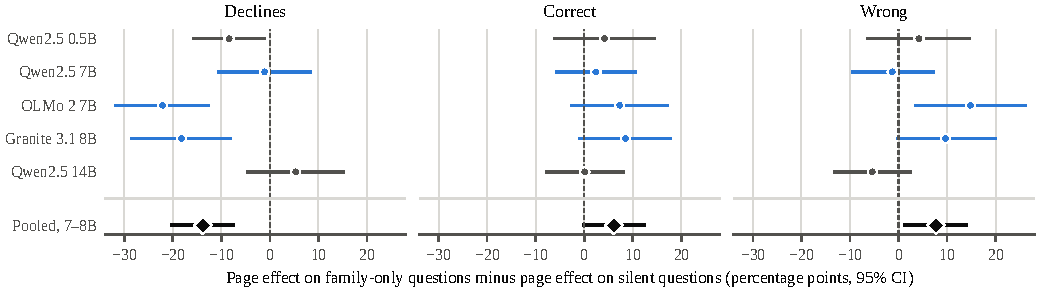
\includegraphics[width=\textwidth]{fig_forest.pdf}
% \caption{What a family-only page does, relative to a silent page. For each
% question, the page effect is its outcome with the page minus its outcome
% closed book; the plot shows the mean page effect on family-only questions
% minus that on silent questions, with 95\% bootstrap intervals. The pooled row
% averages each question over the three 7--8B models (481 questions). Gray rows
% are outside the pooled set.}
% \label{fig:forest}
% \end{figure*}

% \paragraph{With the page in hand, models decline less when it names only the
% family.}
% Table~\ref{tab:outcomes} gives outcomes with the page. In all three 7--8B
% models, a family-only page leads to fewer declines than a silent page: 55.3\%
% against 83.8\% for Qwen2.5-7B, 18.1\% against 45.0\% for OLMo~2, and 43.3\%
% against 75.0\% for Granite. The model answers more, and it answers less
% precisely: among answered questions, family-only pages give 45.5--59.4\%
% precision, against 83.7--95.0\% for pages that name the disease.


% \paragraph{The effect is the page's, not the questions'.}
% The raw comparison also reflects differences between the facts in each group.
% With no page, family-only questions already produce more wrong answers than
% silent ones in all three models (32.6\% against 15.6\% for Qwen2.5-7B, 56.7\%
% against 51.2\% for OLMo~2, 33.0\% against 26.2\% for Granite; supplement), so part of the gap in Table~\ref{tab:outcomes} comes from which facts
% fall in which group. Figure~\ref{fig:forest} removes this by comparing each
% question with itself. Pooled over the three
% 7--8B models, a page raises declines by 14.7 points on family-only questions
% and by 28.5 points on silent ones, a difference of 13.8 points (95\% CI
% $-20.3$ to $-7.5$, $p = 3.6\times10^{-5}$), which holds after a Bonferroni
% correction for the three outcomes ($p = 1.1\times10^{-4}$). The freed
% answers split about evenly. A page lowers wrong answers by 11.0 points on
% family-only questions and by 18.8 on silent ones, a difference of 7.7 points
% (95\% CI 1.2 to 14.0, $p = 0.019$; 0.056 after correction), and it lowers
% correct answers by 3.7 and 9.8 points, a difference of 6.1 points (95\% CI
% $-0.1$ to 12.4, $p = 0.058$). The decline effect is individually significant
% for OLMo~2 ($-22.1$ points, $p = 6\times10^{-6}$) and Granite ($-18.2$ points,
% $p = 0.0006$). Qwen2.5-7B shows no difference in its page effect ($-1.1$
% points, $p = 0.82$): it already declines family-only questions less often
% without a page (32.1\% against 59.4\%), and the page
% raises declines by the same amount in both groups.

% \paragraph{Robustness.}
% The raw pattern holds for both relations in all three models (per-relation
% rates in the supplement), and the 0.5B model shows the decline effect as well
% ($-8.4$ points, 95\% CI $-15.7$ to $-1.1$, $p = 0.027$).

% The decline effect depends on how large the named family is. Splitting the
% family-only questions into thirds by the number of members, the pooled effect is
% $-17.3$ points (95\% CI $-26.2$ to $-8.2$) for families of up to 10 members
% and $-18.4$ ($-26.6$ to $-10.3$) for 11--20 members, but only $-6.5$
% ($-15.7$ to $+3.0$) for larger families (Figure~\ref{fig:fixes}c). A narrow
% family makes the page look answerable.

% \subsection{The Family Name Causes \clade{}}

% \begin{figure}[t]
% \centering
% 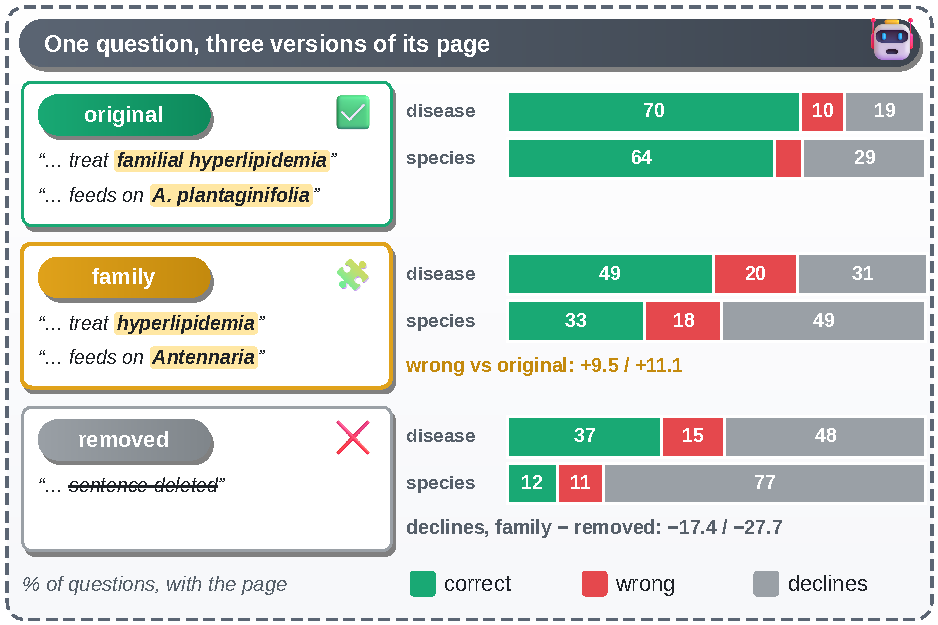
\includegraphics[width=\columnwidth]{fig_edit.pdf}
% \caption{Counterfactual page edit on the same named questions, for diseases
% (PrimeKG, 130 questions) and species (GloBI, 255). \emph{Family} replaces every
% mention of the answer with its parent; \emph{removed} deletes the sentences
% that mention it. Outcomes with the page (\%), averaged over three 7--8B
% models.}
% \label{fig:edit}
% \end{figure}

% The comparison above is between different facts. To hold the fact fixed, we
% edit the page itself. For the 130 named questions whose answer has a parent in
% MONDO, we build two versions of each page: \emph{family} replaces every mention
% of the answer with its parent's name, and \emph{removed} deletes the sentences
% that mention it. Question, options and model are unchanged; only the page
% differs.

% Figure~\ref{fig:edit} shows the result. Relative to the original page, the
% family version lowers correct answers by 21.0 points (95\% CI $-26.9$ to
% $-15.6$) and raises wrong answers by 9.5 (5.9 to 13.6), while declines rise by
% only 11.5 (7.4 to 15.9). Relative to deleting the mention, keeping the family
% name lowers declines by 17.4 points ($-23.6$ to $-11.5$) and raises both wrong
% answers, by 5.1 points (0.5 to 10.3), and correct ones, by 12.3 (6.9 to
% 17.9). Each model shows the same order: Qwen2.5-7B declines 70.0\% of the
% removed versions and 43.8\% of the family versions, Granite 56.2\% and
% 40.8\%, OLMo~2 18.5\% and 7.7\%. The family name therefore produces both
% effects seen in the observational comparison: it suppresses declining, and the
% answers it frees split between right and wrong.

% \subsection{Three Easy Fixes Leave \clade{} in Place}

% \begin{figure*}[t]
% \centering
% \includegraphics[width=\textwidth]{fig_fixes.pdf}
% \caption{Three easy fixes. (a) Confidence separates right from wrong answers
% less well on family-only pages in every model. (b) An instruction to decline
% when the page names only a broad category raises declines on every kind of page
% (pooled over three 7--8B models, 95\% CIs). (c) The decline effect of a
% family-only page is concentrated in small and medium families.}
% \label{fig:fixes}
% \end{figure*}


% \paragraph{Confidence does not flag these answers.}
% A system could answer only when the model is confident. Figure~\ref{fig:fixes}a
% shows that confidence separates right from wrong answers less well on
% family-only pages than on named pages in every model (AUROC 0.59--0.72 against
% 0.73--0.87). The wrong answers are confident: the mean probability of a wrong
% choice on a family-only page is 0.77--0.99 for the 7B and larger models, and
% 0.99 for Qwen2.5 14B. A threshold that keeps most correct answers keeps most of
% these wrong ones too.

% \paragraph{Scale does not remove the gap.}
% Qwen2.5 14B is more precise on named pages than any smaller model (96.0\%,
% Table~\ref{tab:outcomes}), but on family-only pages its precision stays at
% 58.4\%, and it gives 14.7 more points of wrong answers on family-only pages than
% on silent ones ($p = 6\times10^{-6}$). Like Qwen2.5-7B, it already declines
% family-only questions less often without a page, and its page effect does not
% differ between the groups ($+5.3$ points, $p = 0.29$).


% \paragraph{An instruction to decline is not targeted.}
% The simplest remedy is to tell the model: if the page names only a broad
% category that contains the answer, choose ``Not enough information.''
% Figure~\ref{fig:fixes}b shows that the instruction raises declines on
% family-only pages by 15.2 points (95\% CI 12.4 to 18.1), but also by 14.0 on silent pages and by 9.1
% on pages that name the answer, where it costs 6.3 points of correct answers
% ($-9.4$ to $-3.5$).
% Precision on family-only pages stays at 47.9--64.9\% after the instruction,
% far below the 89.6--94.7\% the same prompt gives on named pages (per-model
% rates in the supplement). The instruction does not help because the models do
% not tell a family name from an answer.

% \paragraph{What the result means.}
% A silent page pushes a model toward ``not enough information''; a page naming
% only the family pushes it much less, because it is relevant. The answers this
% frees are about as often wrong as right: the family name lets the model guess
% within a smaller space without telling it which member is meant, and a system
% that treats a relevant page as permission to answer will do so at 45--59\%
% precision while citing a relevant source.

% \subsection{\clade{} in a Second Domain: Species Interactions}

% \begin{table}[t]
% \centering
% \footnotesize
% \setlength{\tabcolsep}{3pt}
% \begin{tabular}{lrr}
% \toprule
%  & PrimeKG & GloBI \\
% \midrule
% Questions, pooled (all-sibling) & 481 & 833 \\
% Decline effect, family $-$ silent & $-13.8$ & $-14.3$ \\
% Wrong effect, family $-$ silent & $+7.7$ & $+11.6$ \\
% Precision, named page (\%) & 84--95 & 84--95 \\
% Precision, family-only page (\%) & 45--59 & 22--28 \\
% AUROC, named page & .73--.87 & .82--.86 \\
% AUROC, family-only page & .66--.72 & .52--.68 \\
% Edit: declines, family $-$ removed & $-17.4$ & $-27.7$ \\
% Edit: wrong, family $-$ removed & $+5.1$ & $+6.7$ \\
% Edit: correct, family $-$ original & $-21.0$ & $-30.8$ \\
% \bottomrule
% \end{tabular}
% \caption{The same tests on drug--disease facts (PrimeKG, MONDO) and on
% species interactions (GloBI, taxonomy), for the three 7--8B models. Effects
% in points; ranges are over models. All effects shown have 95\% CIs that
% exclude zero.}
% \label{tab:globi}
% \end{table}

% To test whether the effect depends on medicine or on MONDO, we repeat the
% abstention test and the counterfactual edit on species interactions from
% GloBI \citep{poelen2014globi}. We keep four relations (\emph{eats},
% \emph{preys on}, \emph{parasite of}, \emph{pollinates}) between species,
% use the consumer's Wikipedia article as the page, and use GloBI's taxonomy
% (species, genus, family) in place of MONDO. A page is named if it gives the
% partner's binomial, its abbreviated form or a common name from Wikipedia
% redirects, and family-only if it gives only the genus or family. Wrong options
% are species of the same genus, then of the same family, and never a recorded
% partner. The question set has 75 questions per group and relation (900 in all).

% Exact partners are rarely written down: of 23,694 measured edges, the page
% names the partner species for 3.9\% and only its genus or family for 7.1\%.
% Table~\ref{tab:globi} shows that every result carries over. A page raises
% declines by 12.1 points on silent questions but lowers them by 2.3 on
% family-only ones, a difference of $-14.3$ points ($p = 1.4\times10^{-9}$);
% the freed answers are mostly wrong ($+11.6$ points, $p = 2.5\times10^{-8}$;
% correct $+2.7$, $p = 0.09$). Family-only precision falls to 22--28\%, since
% species of one genus are harder to tell apart than diseases of one family. The
% counterfactual edit is stronger than on PrimeKG: keeping the genus name instead
% of deleting the sentence lowers declines by 27.7 points ($-32.2$ to $-23.5$)
% and raises wrong answers by 6.7 (3.4 to 10.2; Figure~\ref{fig:edit}). Resolvable insufficiency is a
% property of how text names facts that sit in a hierarchy, not of one domain.


% \section{Methodology}

% Our experimental methodology consists of four parts: (1) evaluating how coarse, family-only passages affect model abstention compared to silent and named passages; (2) performing counterfactual edits on passages to isolate the causal effect of the coarse category name; (3) testing whether standard mitigation strategies prevent premature guessing; and (4) evaluating a three-step ontology pipeline designed to recover the fine-grained answer.

% \subsection{Abstention Evaluation Setup}

% \paragraph{Multiple-choice questions with an abstention option.}
% We construct 856 multiple-choice questions from PrimeKG indication and contraindication facts: 300 with a \emph{named} passage, 256 with a \emph{family-only} passage, and 300 with a \emph{silent} passage (150 per relation and group, except for family-only contraindications, where all 106 available facts are used). Each question presents five candidate diseases alongside a sixth abstention option, \emph{Not enough information to tell}, labeled A through F.

% To make sure the options require fine-grained discrimination, we draw incorrect disease options (distractors) from the true answer's local neighborhood in MONDO. We select sibling diseases first (sharing the same parent), then cousin diseases (sharing the same grandparent), and use random diseases only when siblings and cousins are exhausted. We exclude any ancestor or descendant of the true answer, as well as any other disease linked to the drug by the same relation. Because most distractors belong to the same disease family as the true answer, seeing only the coarse family name in the passage does not logically rule them out.

% \paragraph{Passage construction.}
% Every question is evaluated twice: once closed book (no passage) and once open book (with a retrieved passage). Each passage is built from the drug's cleaned Wikipedia article followed by its retrieved PubMed abstracts. We include the first 800 characters of the text plus a 280-character context window around every mention of the target disease or its family, merging overlapping windows and capping total length at 1,800 characters. For silent passages, which have no mentions, this procedure yields the opening section of the drug's article.

% \paragraph{Models and scoring.}
% We evaluate five instruction-tuned open-weight models across three model families and three parameter scales: Qwen2.5 (0.5B, 7B, and 14B; \citealt{qwen2025qwen25}), OLMo~2 7B \citep{olmo2024olmo2}, and Granite~3.1 8B \citep{granite2024}. Models receive the passage, question, and six options A--F, and we select the option letter with the highest next-token probability (renormalized over the six option letters). We record an outcome as \emph{declined} (abstained) whenever the model selects \emph{Not enough information to tell}.

% \paragraph{Controlling for distractor difficulty and baseline fact hardness.}
% Two potential confounders could bias a naive comparison across passage types. First, family-only questions more frequently have enough relatives in MONDO to fill all four distractor slots with close neighbors, making those questions naturally harder. To eliminate this confounder, our primary analysis restricts all groups to questions where all four distractors come from the answer's MONDO neighborhood (106 named, 215 family-only, and 160 silent questions; full-sample results on all 856 questions appear in the supplement and show the same patterns).

% Second, different passage groups contain different underlying facts, which may vary in baseline difficulty even before a passage is read. We remove this baseline difference using a within-question difference-in-differences design. For each question, we first compute its \emph{page effect}: the outcome when given the passage minus the outcome when asked closed book. We then compare the mean page effect on family-only questions against the mean page effect on silent questions. Confidence intervals are estimated via 5,000 bootstrap resamples at the question level. When pooling across the three 7--8B models, we average each question's page effect across the three models before comparing groups so that each question receives equal weight.

% \subsection{Counterfactual Page Edits and Mitigation Tests}

% \paragraph{Counterfactual text edits.}
% Even with within-question controls, observational groups still test different sets of facts. To hold the underlying question and fact completely constant, we take the 130 named questions whose target disease has a MONDO parent and create two edited versions of each passage:
% \begin{itemize}
% \item \textbf{Family edit:} Every mention of the specific target disease in the passage is replaced with the name of its immediate MONDO parent category.
% \item \textbf{Removed edit:} Every sentence mentioning the target disease is deleted from the passage.
% \end{itemize}
% The question, multiple-choice options, and model remain identical; only the passage text changes.

% \paragraph{Three candidate fixes.}
% We test three practical strategies that might curb \clade{}:
% \begin{enumerate}
% \item \emph{Confidence thresholding:} Using the model's renormalized probability for its chosen answer to filter out uncertain guesses, measured via the area under the ROC curve (AUROC) for separating correct from wrong answers.
% \item \emph{Model scaling:} Comparing Qwen2.5 across 0.5B, 7B, and 14B parameters to see whether larger models abstain appropriately on coarse passages.
% \item \emph{Explicit abstention prompting:} Adding a direct instruction to the prompt telling the model to select \emph{Not enough information to tell} whenever the passage mentions only a broad category rather than a specific disease.
% \end{enumerate}

% \paragraph{Cross-domain replication on GloBI.}
% We replicate both the observational abstention experiment and the counterfactual page-edit experiment on 900 species-interaction questions from GloBI (75 questions per passage type across four ecological relations). Distractors are drawn first from species within the same genus, and then from the same family.

% \subsection{Ontology-Guided Recovery Pipeline}

% To test whether a symbolic ontology can resolve coarse passages into exact answers, we evaluate 410 PrimeKG indication and contraindication facts whose combined Wikipedia and PubMed text mentions only the disease family. Because a single drug often treats or is contraindicated for multiple related diseases within the same family (an average of 2.47 true diseases per family list), we count a recovered candidate as correct if it matches any true disease linked to that drug under the target relation.

% We decompose ontology-based recovery into three stages:
% \begin{enumerate}
% \item \textbf{Identifying the family and listing candidates:} We compare an oracle \emph{given-family} list (which takes the narrowest MONDO ancestor mentioned in the text and expands its descendants up to two levels down, capped at 64 candidates) against an automated \emph{page-built} list (which extracts every MONDO parent category mentioned in the drug's Wikipedia article and takes the union of their descendants, marking lists over 64 candidates as too broad).
% \item \textbf{Scoring and selecting a candidate:} Within the candidate list, we compare five selection methods: (a) Qwen2.5-7B scoring candidates closed book; (b) Qwen2.5-7B scoring candidates with the passage in the prompt; (c) Wikipedia reverse lookup (checking whether the candidate disease's own Wikipedia article mentions the drug); (d) PubMed co-mention counts (the number of PubMed abstracts mentioning both the drug and the candidate disease alongside relation-specific keywords, both raw and normalized by the disease's total PubMed volume); and (e) a simple \emph{popularity prior} that picks the candidate disease with the highest total number of PubMed abstracts regardless of the drug.
% \item \textbf{Non-ontology baselines:} We compare against two baselines that do not use MONDO: a list of the same length containing the true answer mixed with random diseases, scored by the model either with or without the passage in the prompt. Paired accuracy differences are evaluated using McNemar's test \citep{mcnemar1947}.
% \end{enumerate}







\section{Methodology}

We run four experiments. We measure how family-only pages change abstention, edit pages to isolate the effect of the family name, test three common fixes, and test whether an ontology can recover the exact answer.

\subsection{Abstention Evaluation Setup}
\label{subsec:abstention}

\paragraph{Questions.}
We curate 856 multiple-choice questions from the PrimeKG indications and contraindications: 300 with a \emph{named} page, 256 with a \emph{family-only} page, and 300 with a \emph{silent} page. Each relation and group has 150 questions, except family-only contraindications, where only 106 facts exist. Each question has five candidate diseases and a sixth option, \emph{Not enough information to tell}. The four wrong options come from the answer's MONDO neighborhood: siblings first, then cousins, then random diseases only if both run out. We exclude the answer's ancestors and descendants and any other disease the drug has under the same relation. 

\paragraph{Pages.}
We ask each question twice: closed book and with a page. The page starts with the drug's cleaned Wikipedia article, followed by its PubMed abstracts. We keep the first 800 characters and a 280 character window around each mention of the answer or its family, merge overlapping windows, and cap the page at \num{1800} characters. A silent page has no mentions, so it is the article's opening.

\paragraph{Models and Scoring.}
We evaluate five instruction-tuned open-weight models from three families: Qwen2.5 0.5B, 7B and 14B \citep{qwen2025qwen25}, OLMo~2 7B \citep{olmo2024olmo2}, and Granite~3.1 8B \citep{granite2024}. The model sees the page, the question and options A--F. We take the letter with the highest next-token probability, renormalized over the six letters. Choosing \emph{Not enough information to tell} counts as a decline. As a format check, we also ask 120 matched questions with no options and score each generated answer by name matching.

\paragraph{Controls.}
Two differences between groups could bias the comparison. First, family-only answers more often have enough relatives to fill all four wrong options, which makes those questions harder. Our main analysis therefore keeps only questions whose four wrong options all come from the neighborhood: 106 named, 215 family-only and 160 silent. Appendix~D reports all 856 questions, with the same pattern.

Second, the groups hold different facts, which may differ in difficulty before any page is read. We therefore compare each question with itself. For a question $q$ and an outcome such as a decline, let $y_q^{\text{page}}=1$ if the outcome occurs when the model reads the page and $0$ otherwise, and let $y_q^{\text{closed}}$ be the same without the page. The \emph{page effect} of $q$ is $y_q^{\text{page}}-y_q^{\text{closed}}$. Our main measure is the difference in mean page effect between the family-only questions $F$ and the silent questions $S$:
{\setlength{\abovedisplayskip}{3pt}\setlength{\belowdisplayskip}{3pt}%
\begin{equation}
\Delta = \frac{1}{|F|}\sum_{q\in F}\bigl(y_q^{\text{page}}-y_q^{\text{closed}}\bigr) - \frac{1}{|S|}\sum_{q\in S}\bigl(y_q^{\text{page}}-y_q^{\text{closed}}\bigr).
\label{eq:did}
\end{equation}}
For declines, $\Delta<0$ means a family-only page pushes the model toward declining less than a silent page does. To pool the 7--8B models, we average each question's page effect over the models first, so each question counts once.

\paragraph{Statistics.}
Effects are in percentage points. Brackets give 95\% confidence intervals (CI) from 5,000 bootstrap resamples of questions; an interval that excludes \num{0} marks a reliable effect. $p$-values come from two-sided $z$-tests (Appendix~C).

\subsection{Counterfactual Evaluation}

\paragraph{Page edits.}
The groups in~\cref{subsec:abstention} test different facts. To hold the fact fixed, we take 130 named questions whose answer has a MONDO parent. Then we edit each page in two ways: \emph{family edit} replaces every mention of the answer with its parent's name, and \emph{removed edit} deletes every sentence that mentions the answer (\cref{fig:edit}). The question, options and model stay the same.

\paragraph{Simple fixes fail.}
We test three ways to curb \clade{}. \emph{Confidence filtering} uses the renormalized probability of the chosen option; we report the AUROC for separating correct from wrong answers. \emph{Scaling} compares Qwen2.5 at 0.5B, 7B and 14B. \emph{Instruction} adds a line to the prompt telling the model to choose \emph{Not enough information to tell} when the page names only a broad category.

\paragraph{Second domain.}
We repeat the main experiment and counterfactual edits on 900 GloBI questions: 75 per page type in each of four relations. Wrong options come from the same genus first, then the same family.

\subsection{Ontology Recovery}

We test recovery on 410 PrimeKG facts whose Wikipedia and PubMed text names only the disease family (Figure~\ref{fig:concept}). A drug often has several true diseases in a family (2.47 per list on average), so a pick counts as correct if it matches any of them. Recovery has three stages:

\begin{enumerate}
\item \textbf{Build the list.} The oracle \emph{given-family} list takes the narrowest MONDO ancestor named in the text and lists its descendants up to two levels down, capped at 64. The automatic \emph{page-built} list takes every MONDO parent named in the drug's Wikipedia article and joins their descendants; lists over 64 count as too broad. The \emph{model-chosen} list asks Qwen2.5-7B which of the families on the page (up to ten) holds the answer and expands only that one.
\item \textbf{Choose one.} We compare five options: (1) Qwen2.5-7B closed book, (2) Qwen2.5-7B with the page in the prompt, (3) a reverse lookup to check whether the candidate's own Wikipedia article names the drug, (4) PubMed co-mention counts with relation keywords, raw and normalized by the disease's PubMed volume, and (5) a \emph{popularity prior} that picks the disease with the most PubMed abstracts, ignoring the drug.
\item \textbf{Compare without ontology.} Two baselines replace the family list with a list of the same length that holds the answer plus random diseases, scored by the model with or without the page. We test paired differences with McNemar's test \citep{mcnemar1947}.
\end{enumerate}




\section{Results}

\subsection{Coarse evidence weakens abstention (\clade{})}

\begin{table}[t]
\centering
\small
\setlength{\tabcolsep}{2.9pt}
\begin{tabular}{llcccc}
\toprule
Model & Passage Type & Correct & Wrong & Declines & Prec. \\
\midrule
\multirow{3}{*}{Qwen2.5 7B} & named & 71.7 & 3.8 & 24.5 & 95.0 \\
 & family-only & 26.5 & 18.1 & 55.3 & 59.4 \\
 & silent & 13.8 & 2.5 & 83.8 & 84.6 \\
\midrule
\multirow{3}{*}{OLMo 2 7B} & named & 77.4 & 15.1 & 7.5 & 83.7 \\
 & family-only & 37.2 & 44.7 & 18.1 & 45.5 \\
 & silent & 30.6 & 24.4 & 45.0 & 55.7 \\
\midrule
\multirow{3}{*}{Granite 3.1 8B} & named & 72.6 & 7.5 & 19.8 & 90.6 \\
 & family-only & 30.2 & 26.5 & 43.3 & 53.3 \\
 & silent & 15.0 & 10.0 & 75.0 & 60.0 \\
\midrule
\multirow{3}{*}{Qwen2.5 0.5B} & named & 77.4 & 14.2 & 8.5 & 84.5 \\
 & family-only & 34.4 & 55.8 & 9.8 & 38.1 \\
 & silent & 28.7 & 50.6 & 20.6 & 36.2 \\
\midrule
\multirow{3}{*}{Qwen2.5 14B} & named & 67.9 & 2.8 & 29.2 & 96.0 \\
 & family-only & 24.2 & 17.2 & 58.6 & 58.4 \\
 & silent & 11.9 & 2.5 & 85.6 & 82.6 \\
\bottomrule
\end{tabular}
\caption{Open-book outcomes (\%) on PrimeKG questions where all four distractors come from the answer's MONDO neighborhood (106 named, 215 family-only, and 160 silent questions). Precision is the percentage of correct answers among questions where the model did not abstain.}
\label{tab:outcomes}
\end{table}

\begin{figure}[t]
\centering
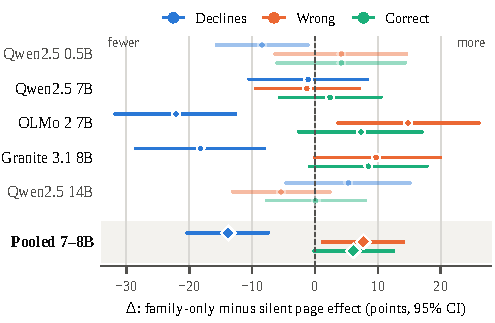
\includegraphics[width=\columnwidth]{figures/fig_forest.pdf}
\caption{Effect of a family-only page relative to a silent page. Each point is $\Delta$ from Eq.~\ref{eq:did} for one outcome, with its 95\% bootstrap CI; points left of zero mean the family-only page lowers that outcome. The pooled row averages the three 7-8B models over 481 questions. Faded rows are models outside the pooled set.}
\label{fig:forest}
\end{figure}

\paragraph{Models abstain less with partial evidence.}
\Cref{tab:outcomes} shows outcomes when the model reads the page. All 7-8B models abstain much less on a family-only page than on a silent page: Qwen2.5-7B from 83.8\% to 55.3\%, OLMo~2 from 45.0\% to 18.1\%, and Granite from 75.0\% to 43.3\%. Many of the extra answers are wrong. Precision, the share of answers that are correct, falls from 83.7-95.0\% on named pages to 45.5-59.4\% on family-only pages.

\paragraph{\clade{} drop comes from context.}
Family-only facts are harder even closed book: they draw more wrong guesses than silent facts in all three 7-8B models (Appendix~D). The page effect in Eq.~\ref{eq:did} removes this difference. Pooled over the models, a silent page raises abstention by $28.5$ points over closed book, but a family-only page raises them by only 14.7 points. The difference $\Delta$ is $-13.8$ points [$-20.3$, $-7.5$], and it stays significant after a Bonferroni correction for three outcomes ($p$=1.1$\times10^{-4}$; \cref{fig:forest}). The freed answers split between wrong answers ($+7.7$ [$1.2$, $14.0$]) and correct ones ($+6.1$ [$-0.1$, $12.4$]). In plain terms, a silent page makes the models stop and say they cannot tell; a family-only page makes them stop much less often, and they guess instead. The drop is significant for OLMo~2 ($-22.1$, $p$=6$\times10^{-6}$), Granite ($-18.2$, $p$=6$\times10^{-4}$) and Qwen2.5-0.5B ($-8.4$, $p$=$0.027$). Qwen2.5-7B shows almost no gap ($-1.1$, $p$=$0.82$). It already declines family-only questions far less often closed book (32.1\% vs.\ 59.4\%), and the page raises its abstention by about the same amount in both groups.

\paragraph{An example.}
For moxifloxacin, PrimeKG lists \emph{Klebsiella pneumonia}, and the page says only that the drug treats pneumonia. All five models pick some bacterial pneumonia with confidence up to 1.00, and none abstains. For lovastatin, OLMo~2 is right closed book but picks a sibling after reading a page that says only \emph{hyperlipidemia} (Appendix~I).

\paragraph{Family size.}
We split the family-only questions into thirds by family size. The drop is large for families of up to 10 members ($-17.3$ [$-26.2$, $-8.2$]) and of 11-20 members ($-18.4$ [$-26.6$, $-10.3$]). It shrinks to $-6.5$ [$-15.7$, $+3.0$] for families above 20 members (\cref{fig:fixes}c). A narrow family makes the page look more answerable.

\subsection{Counterfactual Edits confirm \clade{}}

\begin{figure}[t]
\centering
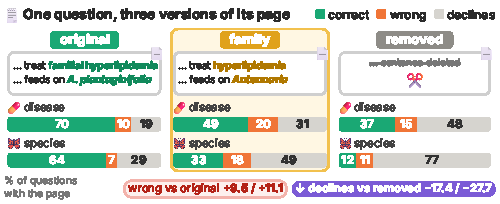
\includegraphics[width=\columnwidth]{figures/fig_example.pdf}
\caption{Page edits on the same questions: PrimeKG (130) and GloBI (255). The \emph{family} edit replaces the answer with its parent; the \emph{removed} edit deletes the sentence. Bars show outcomes with the page (\%), averaged over the 7-8B models.}
\label{fig:edit}
\end{figure}

The edits change only the page (\cref{fig:edit}). Against the original page, the family edit lowers correct answers by 21.0 points and raises wrong answers by 9.5 points, while abstention rises by only 11.5 points. The key comparison is with the removed edit. Keeping the family name instead of deleting the sentence cuts abstention by 17.4 points [$-23.6$, $-11.5$] and raises wrong answers by 5.1 points [$0.5$, $10.3$]. Every model shows this order: from removed to family, abstention falls from 70.0\% to 43.8\% for Qwen2.5-7B, from 56.2\% to 40.8\% for Granite, and from 18.5\% to 7.7\% for OLMo~2. The family name alone suppresses abstention.

\subsection{Three Fixes Fall Short}

\begin{figure*}[t]
\centering
\includegraphics[width=\textwidth]{figures/fig_fixes.pdf}
\caption{Three candidate fixes. (a) Confidence separates correct from wrong answers poorly on family-only pages. (b) An instruction to decline on broad categories raises abstention on every page type, including named pages (pooled 7-8B models, 95\% CIs). (c) The drop in abstention is largest when the family has 20 or fewer members.}
\label{fig:fixes}
\end{figure*}

\paragraph{Confidence does not flag wrong answers.}
AUROC measures how well confidence ranks the correct answers above wrong ones: 1.0 is perfect and 0.5 is chance. On family-only pages it is 0.59-0.72, against 0.73-0.87 on named pages, in every model (\cref{fig:fixes}a). Wrong guesses are confident: their mean probability is 0.77-0.99 in 7-14B models. A threshold that keeps correct answers also keeps most wrong ones.

\paragraph{Scaling does not help.}
Qwen2.5-14B has the best precision on named pages (96.0\%). On family-only pages, precision rises from 38.1\% at 0.5B to 59.4\% at 7B, but then stops: 14B reaches 58.4\%, and it gives 14.7 points more wrong answers than on silent pages ($p$=6$\times10^{-6}$).

\paragraph{Instruction.}
Telling the model not to answer when the page names only a broad category raises abstention by 15.2 points on family-only pages (\cref{fig:fixes}b). It also raises them by 14.0 points on silent pages and 9.1 points on named pages, where it costs 6.3 points of correct answers. Precision on family-only pages stays at 47.9-64.9\%, far below named pages (89.6-94.7\%). The models scores change differently, OLMo~2 abstains far more on all page types, while Granite barely changes (Appendix~F). However, none of these models tells a family name from a specific answer.

\subsection{Second Domain: GloBI}

\begin{table}[t]
\centering
\footnotesize
\setlength{\tabcolsep}{2.6pt}
\begin{tabular}{lrr}
\toprule
Metric & PrimeKG & GloBI \\
\midrule
Questions in pooled set (all-neighbor) & 481 & 833 \\
Abstention page effect, family $-$ silent & $-13.8$ & $-14.3$ \\
Wrong-answer page effect, family $-$ silent & $+7.7$ & $+11.6$ \\
Precision on named passages (\%) & 84--95 & 84--95 \\
Precision on family-only passages (\%) & 45--59 & 22--28 \\
Confidence AUROC on named passages & .73--.87 & .82--.86 \\
Confidence AUROC on family-only passages & .66--.72 & .52--.68 \\
Edit: abstention, family $-$ removed & $-17.4$ & $-27.7$ \\
Edit: wrong answers, family $-$ removed & $+5.1$ & $+6.7$ \\
Edit: correct answers, family $-$ original & $-21.0$ & $-30.8$ \\
\bottomrule
\end{tabular}
\caption{Comparison of biomedical drug--disease facts (PrimeKG with MONDO) and ecological species interactions (GloBI with biological taxonomy) across the three 7--8B models. Effects are reported in percentage points; ranges span individual models. Every difference reported has a 95\% CI excluding zero.}
\label{tab:globi}
\end{table}

Every finding on PrimeKG replicates on species interactions (\cref{tab:globi}). A silent page raises abstention by 12.1 points, but a page that names only the genus or family lowers them by 2.3 points ($\Delta$=$-14.3$, $p$=1.4$\times10^{-9}$). The effect is largest in OLMo~2 ($-31.7$). Here the extra answers are mostly wrong ($+11.6$ wrong, $p$=2.5$\times10^{-8}$; $+2.7$ correct, $p$=$0.09$). Precision on family-only pages falls to 22-28\%, close to the 20\% chance rate, because sibling species are harder to tell apart than sibling diseases. The page edit is even sharper: on 255 questions, keeping the genus name instead of deleting the sentence cuts abstention by 27.7 points [$-32.2$, $-23.5$] and raises wrong answers by 6.7 points (\cref{fig:edit}). \clade{} comes from hierarchical evidence in text, not from medical terms (Appendix~G).

\subsection{Ontology Recovery}

\begin{figure}[t]
\centering
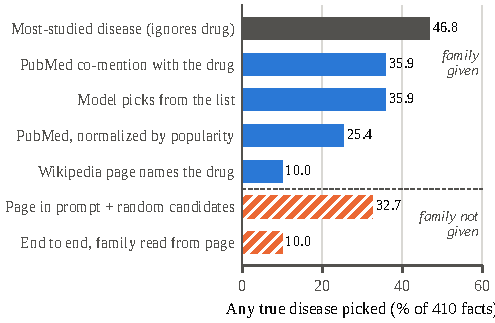
\includegraphics[width=0.9\columnwidth]{figures/fig_recovery.pdf}
\caption{Accuracy of choosing the exact disease for 410 family-only facts. Blue and gray bars choose from the given-family list; hatched bars do not receive the true family.}
\label{fig:recovery}
\end{figure}

\begin{table}[t]
\centering
\small
\setlength{\tabcolsep}{3pt}
\begin{tabular}{@{}lccc@{}}
\toprule
Metric & Given & Page-built & Model-chosen \\
\midrule
Usable lists (of 410) & 410 & 166 & 375 \\
Holds sampled answer & 98.5\% & 19.8\% & 30.0\% \\
Holds any true answer & 99.5\% & 24.6\% & 44.9\% \\
Median list size & 14 & 32 & 12 \\
End-to-end recovery & -- & 10.0\% & 26.8\% \\
\bottomrule
\end{tabular}
\caption{Candidate lists for the 410 family-only facts: given family (oracle), all families on the page (page-built), and the one family Qwen2.5-7B picks from the page (model-chosen). Of the 244 unusable page-built lists, 209 exceed the 64-candidate cap and 35 match no multi-child MONDO family. End-to-end recovery uses the best chooser for each list.}
\label{tab:lists}
\end{table}

\paragraph{List coverage.}
When the right family is given, its MONDO descendants form a list of median 14 candidates. The list holds the sampled answer 98.5\% of the time and some true answer 99.5\% of the time (\cref{tab:lists}).

\paragraph{Finding the family.}
When the family must come from the drug's Wikipedia page, usable lists hold the answer for only 19.8\% of facts. The family is rarely missing; it is buried. A drug article names a median of five MONDO categories, such as comorbidities, side effects and other uses, and their union exceeds 64 candidates for 209 of 410 facts. PubMed makes this worse: coverage drops to 3.7\%. A model does better than string matching. When Qwen2.5-7B reads the page and picks one of the families it names, the chosen list holds the answer for 30.0\% of facts (44.9\% for any true answer), above the first-mentioned family (25.1\%) and a random one (13.9\%). The ceiling is 50.0\%: for half of the facts, the right family is not among the usable families on the page.

\paragraph{Choosing a member.}
Within the given-family list (\cref{fig:recovery}), Qwen2.5-7B alone reaches 35.9\% (32.4\% with the page in the prompt), and raw PubMed co-mentions also reach 35.9\%. Evidence first, with the model as a fallback, reaches 41.7\%. Yet the best chooser ignores the drug: picking the disease with the most PubMed abstracts reaches 46.8\%. When we divide co-mentions by each disease's abstract count, accuracy drops from 35.9\% to 25.4\%, so co-mentions work mainly because common diseases are studied more.

\paragraph{Errors and end-to-end recovery.}
Most misses pick a better-studied sibling, such as \emph{ovarian carcinoma} instead of \emph{malignant germ cell tumor of ovary} for carboplatin, or a valid use missing from PrimeKG, so strict graph scoring understates accuracy (Appendix~H). Without the given family, page-built lists recover the answer for 10.0\% of facts with Wikipedia and 1.5\% with PubMed added; model-chosen lists recover 26.8\% (\cref{tab:lists}).


\section{Discussion}

\paragraph{Hand-off point.}
Our results mark a clear boundary between the language model and the ontology. On a family-only page, models take the family as license to guess. The ontology turns the same family into a short list that holds the answer, once the system knows which family on the page belongs to the question.

\paragraph{A three-step workflow.}
This suggests a simple workflow (\cref{fig:concept}). (1)~\textbf{Check the page type}, and answer from the page only if it names the answer. (2)~\textbf{Find the target family} tied to the queried relation; if none fits, abstain. (3)~\textbf{Expand and choose} with evidence and a popularity prior; answer only when one candidate clearly leads, otherwise return the list. Current models skip steps 1 and 2, and neither confidence nor instructions restore step~1. Step~2 is the main bottleneck: string matching finds the right family for 19.8\% of facts, and a model chooser raises this to 30.0\%, against a ceiling of 50.0\%. Any chooser for step~3 should beat the popularity prior.

\paragraph{Beyond sufficiency.}
Recent work asks whether a page is sufficient \citep{joren2025sufficient}; our results show that \emph{how} it falls short matters. A family-only page differs from a silent one: it carries real signal, it breaks abstention, and it points into a symbolic hierarchy. Treating it as its own case lets a RAG system send partial evidence to an ontology instead of guessing or discarding it.

\section{Limitations}

We study two domains and run recovery only on PrimeKG. We use multiple-choice questions with an explicit decline option, which controls the wrong options and the scoring but may differ from free-text refusals. A free-text check points the same way (Appendix~K): no model gives the exact answer from a family-only page, and 17.5--45.0\% of its answers name the family itself. We test open models up to 14B, and the page edits cover only named facts whose answer has a parent. Page-built lists rely on exact string matching. Family-only contraindications are few (106 questions).

\section{Conclusion}

Retrieved text often states facts at a coarser level than the question asks. We show that this \emph{resolvable insufficiency} triggers \clade{} in medicine and ecology: a family or genus name leads models to stop declining and guess, which roughly halves precision. An ontology can narrow the answer to a short list that holds it 98.5\% of the time once the right family is found, and a model that chooses the family from the page already raises end-to-end recovery from 10.0\% to 26.8\%. Finding the family more reliably and beating a popularity prior remain the key open problems for neuro-symbolic RAG.


\bibliography{main}

\end{document}